%%% Local Variables:
%%% mode: latex
%%% TeX-master: t
%%% End:

\documentclass[bachelor,xetex,openany]{thuthesis}
% \documentclass[%
%   bachelor|master|doctor, % mandatory option
%   xetex|pdftex|dvips|dvipdfm, % optional
%   secret,
%   openany|openright,
%   arialtoc,arialtitle]{thuthesis}

% 所有其它可能用到的包都统一放到这里了,可以根据自己的实际添加或者删除。
\usepackage{thutils}

% 你可以在这里修改配置文件中的定义,导言区可以使用中文。
\def\myname{冯时}

\begin{document}

% 定义所有的eps文件在 figures 子目录下
\graphicspath{{figures/}}


%%% 封面部分
\frontmatter
\ctitle{分布式二级哈希表}
% 根据自己的情况选,不用这样复杂
\cdegree{工学硕士}
\cdepartment[计算机]{计算机科学与技术系}
\cmajor{计算机科学与技术}
\cauthor{冯时} 
\csupervisor{陈文光教授}
% 如果没有副指导老师或者联合指导老师,把下面两行相应的删除即可。
\cassosupervisor{陈康副教授}
% 日期自动生成,如果你要自己写就改这个cdate
%\cdate{\CJKdigits{\the\year}年\CJKnumber{\the\month}月}

% 定义中英文摘要和关键字
\begin{cabstract}
随着互联网的发展和云存储的兴起,传统的分布式哈希表越来越难以满足丰富的个人在线
存储应用对存储后端的需求。二级哈希表存储的是具有二级索引的数据,因此能够提供更
丰富的语义。本论文阐述了分布式二级哈希表的架构设计和实现细节,说明了性能对于分
布式存储系统的重要性。分布式二级哈希表综合了分布式系统领域的一些经典技术,利用
配置服务器集中管理控制信息,并采用一致性哈希进行数据的分配和备份。
\end{cabstract}

\ckeywords{分布式, 哈希表, 存储, 性能, 一致性哈希}

\begin{eabstract} 
With the development of Internet and boom of cloud storage, traditional
distributed hash table is too simple to support the upper layer applications
which provide personal online storage service. A two-level DHT stores data
with a major index plus a secondary one, resulting in more complex semantics.
The present thesis describes both architecture design and implementation
details of two-level DHTs, and comes to a conclusion that high performance and
efficiency is fundamental aspect of a distributed system. The two-level DHT is
a combination of classical technologies in distribute computing, with a config
server to monitor the cluster. It also employs consistent hashing to solve
data partition and replication.
\end{eabstract}

\ekeywords{distributed, hash table, storage, performance, consistent hashing}

\makecover

% 目录
\tableofcontents

% 符号对照表
%\begin{denotation}

\item[HPC] 高性能计算 (High Performance Computing)
\item[cluster] 集群
\item[Itanium] 安腾
\item[SMP] 对称多处理
\item[API] 应用程序编程接口
\item[PI]	聚酰亚胺
\item[MPI]	聚酰亚胺模型化合物,N-苯基邻苯酰亚胺
\item[PBI]	聚苯并咪唑
\item[MPBI]	聚苯并咪唑模型化合物,N-苯基苯并咪唑
\item[PY]	聚吡咙
\item[PMDA-BDA]	均苯四酸二酐与联苯四胺合成的聚吡咙薄膜
\item[$\Delta G$]  	活化自由能~(Activation Free Energy)
\item [$\chi$] 传输系数~(Transmission Coefficient)
\item[$E$] 能量
\item[$m$] 质量
\item[$c$] 光速
\item[$P$] 概率
\item[$T$] 时间
\item[$v$] 速度
\item[劝  学] 君子曰:学不可以已。青,取之于蓝,而青于蓝;冰,水为之,而寒于水。
  木直中绳。(车柔)以为轮,其曲中规。虽有槁暴,不复挺者,(车柔)使之然也。故木
  受绳则直, 金就砺则利,君子博学而日参省乎己,则知明而行无过矣。吾尝终日而思
  矣,  不如须臾之所学也;吾尝(足齐)而望矣,不如登高之博见也。登高而招,臂非加
  长也,  而见者远;  顺风而呼,  声非加疾也,而闻者彰。假舆马者,非利足也,而致
  千里;假舟楫者,非能水也,而绝江河,  君子生非异也,善假于物也。积土成山,风雨
  兴焉;积水成渊,蛟龙生焉;积善成德,而神明自得,圣心备焉。故不积跬步,无以至千
  里;不积小流,无以成江海。骐骥一跃,不能十步;驽马十驾,功在不舍。锲而舍之,朽
  木不折;  锲而不舍,金石可镂。蚓无爪牙之利,筋骨之强,上食埃土,下饮黄泉,用心
  一也。蟹六跪而二螯,非蛇鳝之穴无可寄托者,用心躁也。\pozhehao{} 荀况
\end{denotation}



%%% 正文部分
\mainmatter

%%% Local Variables:
%%% mode: latex
%%% TeX-master: t
%%% End:

\chapter{引言}
\label{cha:intro}

分布式存储系统越来越成为整个互联网得以存在和发展的强大依托。
分布式系统是将多个计算或存储单元通过网络连接整合在一起,共同完成一个任务的系
统。组成分布式系统的每一个计算或存储单元,既可能是不可分割的单一单元,也可能是
另一个分布式系统。组成分布式系统的各个单元协同工作,使得整个系统获得了更高的计
算效率和更大的存储空间。当然,分布式系统的意义远不止如此。

小老鼠偷吃热凉粉;短长虫环绕矮高粱。\footnote{韩愈(768-824),字退之,河南河阳(
  今河南孟县)人,自称郡望昌黎,世称韩昌黎。幼孤贫刻苦好学,德宗贞元八年进士。曾
  任监察御史,因上疏请免关中赋役,贬为阳山县令。后随宰相裴度平定淮西迁刑部侍郎,
  又因上表谏迎佛骨,贬潮州刺史。做过吏部侍郎,死谥文公,故世称韩吏部、韩文公。是
  唐代古文运动领袖,与柳宗元合称韩柳。诗力求险怪新奇,雄浑重气势。}


\section{封面相关}
封面的例子请参看 cover.tex。主要符号表参看 denation.tex,附录和个人简历分别参看 appendix01.tex
和 resume.tex。里面的命令都非常简单,一看即会。\footnote{你说还是看不懂?怎么会呢?}

\section{字体命令}
\label{sec:first}

苏轼(1037-1101),北宋文学家、书画家。字子瞻,号东坡居士,眉州眉山(今属四川)人
。苏洵子。嘉佑进士。神宗时曾任祠部员外郎,因反对王安石新法而求外职,任杭州通判,
知密州、徐州、湖州。后以作诗“谤讪朝廷”罪贬黄州。哲宗时任翰林学士,曾出知杭州、
颖州等,官至礼部尚书。后又贬谪惠州、儋州。北还后第二年病死常州。南宋时追谥文忠。
与父洵弟辙,合称“三苏”。在政治上属于旧党,但也有改革弊政的要求。其文汪洋恣肆,
明白畅达,为“唐宋八大家”之一。  其诗清新豪健,善用夸张比喻,在艺术表现方面独具
风格。少数诗篇也能反映民间疾苦,指责统治者的奢侈骄纵。词开豪放一派,对后代很有影
响。《念奴娇·赤壁怀古》、《水调歌头·丙辰中秋》传诵甚广。

{\kai 坡仙擅长行书、楷书,取法李邕、徐浩、颜真卿、杨凝式,而能自创新意。用笔丰腴
  跌宕,有天真烂漫之趣。与蔡襄、黄庭坚、米芾并称“宋四家”。能画竹,学文同,也喜
  作枯木怪石。论画主张“神似”,认为“论画以形似,见与儿童邻”;高度评价“诗中有
  画,画中有诗”的艺术造诣。诗文有《东坡七集》等。存世书迹有《答谢民师论文帖》、
  《祭黄几道文》、《前赤壁赋》、《黄州寒食诗帖》等。  画迹有《枯木怪石图》、《
  竹石图》等。}

{\fs 易与天地准,故能弥纶天地之道。仰以观於天文,俯以察於地理,是故知幽明之故。原
  始反终,故知死生之说。精气为物,游魂为变,是故知鬼神之情状。与天地相似,故不违。
  知周乎万物,而道济天下,故不过。旁行而不流,乐天知命,故不忧。安土敦乎仁,故
  能爱。范围天地之化而不过,曲成万物而不遗,通乎昼夜之道而知,故神无方而易无体。}

{\you 有天地,然后万物生焉。盈天地之间者,唯万物,故受之以屯;屯者盈也,屯者物之
  始生也。物生必蒙,故受之以蒙;蒙者蒙也,物之穉也。物穉不可不养也,故受之以需;
  需者饮食之道也。饮食必有讼,故受之以讼。讼必有众起,故受之以师;师者众也。众必
  有所比,故受之以比;比者比也。比必有所畜也,故受之以小畜。物畜然后有礼,故受之
  以履。}

{\hei 履而泰,然后安,故受之以泰;泰者通也。物不可以终通,故受之以否。物不可以终
  否,故受之以同人。与人同者,物必归焉,故受之以大有。有大者不可以盈,故受之以谦。
  有大而能谦,必豫,故受之以豫。豫必有随,故受之以随。以喜随人者,必有事,故受
  之以蛊;蛊者事也。}

{\li 有事而后可大,故受之以临;临者大也。物大然后可观,故受之以观。可观而后有所合
  ,故受之以噬嗑;嗑者合也。物不可以苟合而已,故受之以贲;贲者饰也。致饰然后亨
  ,则尽矣,故受之以剥;剥者剥也。物不可以终尽,剥穷上反下,故受之以复。复则不
  妄矣,故受之以无妄。}

{\song 有无妄然后可畜,故受之以大畜。物畜然后可养,故受之以颐;颐者养也。不养则不
  可动,故受之以大过。物不可以终过,故受之以坎;坎者陷也。陷必有所丽,故受之以
  离;离者丽也。}

\section{表格样本}
\label{chap1:sample:table} 

\subsection{基本表格}
\label{sec:basictable}

模板中关于表格的宏包有三个: \textsf{booktabs}、\textsf{array} 和
\textsf{longtabular},命令有一个 \verb|\hlinewd|。三线表可以用 \textsf{booktabs}
提供的 \verb|\toprule|、\verb|\midrule| 和 \verb|\bottomrule|。它们与
\textsf{longtable} 能很好的配合使用。如果表格比较简单的话可以直接用命令
\verb|hlinewd{xpt}| 控制。
\begin{table}[htb]
  \centering
  \begin{minipage}[t]{0.8\linewidth} % 如果想在表格中使用脚注,minipage是个不错的办法
  \caption[模板文件]{模板文件。如果表格的标题很长,那么在表格索引中就会很不美
    观,所以要像 chapter 那样在前面用中括号写一个简短的标题。这个标题会出现在索
    引中。}
  \label{tab:template-files}
    \begin{tabular*}{\linewidth}{lp{10cm}}
      \toprule[1.5pt]
      {\hei 文件名} & {\hei 描述} \\\midrule[1pt]
      thuthesis.ins & \LaTeX{} 安装文件,docstrip\footnote{表格中的脚注} \\
      thuthesis.dtx & 所有的一切都在这里面\footnote{再来一个}。\\
      thuthesis.cls & 模板类文件。\\
      thuthesis.cfg & 模板配置文。cls 和 cfg 由前两个文件生成。\\
      thubib.bst    & 参考文献 Bibtex 样式文件。\\
      thutils.sty   & 常用的包和命令写在这里,减轻主文件的负担。\\
      \bottomrule[1.5pt]
    \end{tabular*}
  \end{minipage}
\end{table}

首先来看一个最简单的表格。表 \ref{tab:template-files} 列举了本模板主要文件及其功
能。请大家注意三线表中各条线对应的命令。这个例子还展示了如何在表格中正确使用脚注。
由于 \LaTeX{} 本身不支持在表格中使用 \verb|\footnote|,所以我们不得不将表格放在
小页中,而且最好将表格的宽度设置为小页的宽度,这样脚注看起来才更美观。

\subsection{复杂表格}
\label{sec:complicatedtable}

我们经常会在表格下方标注数据来源,或者对表格里面的条目进行解释。前面的脚注是一种
不错的方法,如果你不喜欢脚注。那么完全可以在表格后面自己写注释,比如表~\ref{tab:tabexamp1}。
\begin{table}[h]
  \centering
  \caption{复杂表格示例 1}
  \label{tab:tabexamp1}
  \begin{minipage}[t]{0.8\textwidth} 
    \begin{tabularx}{\linewidth}{|l|X|X|X|X|}
      \hline
 \multirow{2}*{\backslashbox{x}{y}}  & \multicolumn{2}{c|}{First Half} & \multicolumn{2}{c|}{Second Half}\\\cline{2-5}
      & 1st Qtr &2nd Qtr&3rd Qtr&4th Qtr \\ \hline
      East$^{*}$ &   20.4&   27.4&   90&     20.4 \\
      West$^{**}$ &   30.6 &   38.6 &   34.6 &  31.6 \\ \hline
    \end{tabularx}\\[2pt]
    \footnotesize 注:数据来源《\thuthesis{} 使用手册》。\\
    *:东部\\
    **:西部
  \end{minipage}
\end{table}

此外,表~\ref{tab:tabexamp1} 同时还演示了另外两个功能:1)通过 \textsf{tabularx} 的
 \texttt{|X|} 扩展实现表格自动放大;2)通过命令 \verb|\backslashbox| 在表头部分
插入反斜线。

为了使我们的例子更接近实际情况,我会在必要的时候插入一些“无关”文字,以免太多图
表同时出现,导致排版效果不太理想。第一个出场的当然是我的最爱:风流潇洒、骏马绝尘、
健笔凌云的{\hei 李太白}了。

李白,字太白,陇西成纪人。凉武昭王暠九世孙。或曰山东人,或曰蜀人。白少有逸才,志
气宏放,飘然有超世之心。初隐岷山,益州长史苏颋见而异之,曰:“是子天才英特,可比
相如。”天宝初,至长安,往见贺知章。知章见其文,叹曰:“子谪仙人也。”言于明皇,
召见金銮殿,奏颂一篇。帝赐食,亲为调羹,有诏供奉翰林。白犹与酒徒饮于市,帝坐沉香
亭子,意有所感,欲得白为乐章,召入,而白已醉。左右以水颒面,稍解,援笔成文,婉丽
精切。帝爱其才,数宴见。白常侍帝,醉,使高力士脱靴。力士素贵,耻之,摘其诗以激杨
贵妃。帝欲官白,妃辄沮止。白自知不为亲近所容,恳求还山。帝赐金放还。乃浪迹江湖,
终日沉饮。永王璘都督江陵,辟为僚佐。璘谋乱,兵败,白坐长流夜郎,会赦得还。族人阳
冰为当涂令,白往依之。代宗立,以左拾遗召,而白已卒。文宗时,诏以白歌诗、裴旻剑舞、
张旭草书为三绝云。集三十卷。今编诗二十五卷。\hfill\pozhehao《全唐诗》诗人小传

浮动体的并排放置一般有两种情况:1)二者没有关系,为两个独立的浮动体;2)二者隶属
于同一个浮动体。对表格来说并排表格既可以像图~\ref{tab:parallel1}、图~\ref{tab:parallel2} 
使用小页环境,也可以如图~\ref{tab:subtable} 使用子表格来做。图的例子参见第~\ref{sec:multifig} 节。
\begin{table}[h]
\noindent\begin{minipage}{0.5\textwidth}
\centering
\caption{第一个并排子表格}
\label{tab:parallel1}
\begin{tabular}{p{2cm}p{2cm}}
\toprule[1.5pt]
111 & 222 \\\midrule[1pt]
222 & 333 \\\bottomrule[1.5pt]
\end{tabular}
\end{minipage}
\begin{minipage}{0.5\textwidth}
\centering
\caption{第二个并排子表格}
\label{tab:parallel2}
\begin{tabular}{p{2cm}p{2cm}}
\toprule[1.5pt]
111 & 222 \\\midrule[1pt]
222 & 333 \\\bottomrule[1.5pt]
\end{tabular}
\end{minipage}
\end{table}

然后就是忧国忧民,诗家楷模杜工部了。杜甫,字子美,其先襄阳人,曾祖依艺为巩令,因
居巩。甫天宝初应进士,不第。后献《三大礼赋》,明皇奇之,召试文章,授京兆府兵曹参
军。安禄山陷京师,肃宗即位灵武,甫自贼中遁赴行在,拜左拾遗。以论救房琯,出为华州
司功参军。关辅饥乱,寓居同州同谷县,身自负薪采梠,餔糒不给。久之,召补京兆府功曹,
道阻不赴。严武镇成都,奏为参谋、检校工部员外郎,赐绯。武与甫世旧,待遇甚厚。乃于
成都浣花里种竹植树,枕江结庐,纵酒啸歌其中。武卒,甫无所依,乃之东蜀就高適。既至
而適卒。是岁,蜀帅相攻杀,蜀大扰。甫携家避乱荆楚,扁舟下峡,未维舟而江陵亦乱。乃
溯沿湘流,游衡山,寓居耒阳。卒年五十九。元和中,归葬偃师首阳山,元稹志其墓。天宝
间,甫与李白齐名,时称李杜。然元稹之言曰:“李白壮浪纵恣,摆去拘束,诚亦差肩子美
矣。至若铺陈终始,排比声韵,大或千言,次犹数百,词气豪迈,而风调清深,属对律切,
而脱弃凡近,则李尚不能历其藩翰,况堂奥乎。”白居易亦云:“杜诗贯穿古今,  尽工尽
善,殆过于李。”元、白之论如此。盖其出处劳佚,喜乐悲愤,好贤恶恶,一见之于诗。而
又以忠君忧国、伤时念乱为本旨。读其诗可以知其世,故当时谓之“诗史”。旧集诗文共六
十卷,今编诗十九卷。

\begin{table}
\centering
\caption{并排子表格}
\label{tab:subtable}
\subfloat[第一个子表格]{
\begin{tabular}{p{2cm}p{2cm}}
\toprule[1.5pt]
111 & 222 \\\midrule[1pt]
222 & 333 \\\bottomrule[1.5pt]
\end{tabular}}\hskip2cm
\subfloat[第二个子表格]{
\begin{tabular}{p{2cm}p{2cm}}
\toprule[1.5pt]
111 & 222 \\\midrule[1pt]
222 & 333 \\\bottomrule[1.5pt]
\end{tabular}}
\end{table}

不可否认 \LaTeX{} 的表格功能没有想象中的那么强大,不过只要你足够认真,足够细致,那么
同样可以排出来非常复杂非常漂亮的表格。请参看表~\ref{tab:tabexamp2}。
\begin{table}[hb]
  \centering\dawu[1.3]
  \caption{复杂表格示例 2}
  \label{tab:tabexamp2}
  \begin{tabular}[c]{|c|m{0.8in}|c|c|c|c|c|}\hline
    \multicolumn{2}{|c|}{Network Topology} & \# of nodes & 
    \multicolumn{3}{c|}{\# of clients} & Server \\\hline
    GT-ITM & Waxman Transit-Stub & 600 &
    \multirow{2}{2em}{2\%}& 
    \multirow{2}{2em}{10\%}& 
    \multirow{2}{2em}{50\%}& 
    \multirow{2}{1.2in}{Max. Connectivity}\\\cline{1-3}
    \multicolumn{2}{|c|}{Inet-2.1} & 6000 & & & &\\\hline
    \multirow{2}{1in}{Xue} & Rui  & Ni &\multicolumn{4}{c|}{\multirow{2}*{\thuthesis}}\\\cline{2-3}
    & \multicolumn{2}{c|}{ABCDEF} &\multicolumn{4}{c|}{} \\\hline
\end{tabular}
\end{table}

最后就是清新飘逸、文约意赅、空谷绝响的王大侠了。王维,字摩诘,河东人。工书画,与
弟缙俱有俊才。开元九年,进士擢第,调太乐丞。坐累为济州司仓参军,历右拾遗、监察御
史、左补阙、库部郎中,拜吏部郎中。天宝末,为给事中。安禄山陷两都,维为贼所得,服
药阳喑,拘于菩提寺。禄山宴凝碧池,维潜赋诗悲悼,闻于行在。贼平,陷贼官三等定罪,
特原之,责授太子中允,迁中庶子、中书舍人。复拜给事中,转尚书右丞。维以诗名盛于开
元、天宝间,宁薛诸王驸马豪贵之门,无不拂席迎之。得宋之问辋川别墅,山水绝胜,与道
友裴迪,浮舟往来,弹琴赋诗,啸咏终日。笃于奉佛,晚年长斋禅诵。一日,忽索笔作书
数纸,别弟缙及平生亲故,舍笔而卒。赠秘书监。宝应中,代宗问缙:“朕常于诸王坐闻维
乐章,今存几何?”缙集诗六卷,文四卷,表上之。敕答云,卿伯氏位列先朝,名高希代。
抗行周雅,长揖楚辞。诗家者流,时论归美。克成编录,叹息良深。殷璠谓维诗词秀调雅,
意新理惬。在泉成珠,著壁成绘。苏轼亦云:“维诗中有画,画中有诗也。”今编诗四卷。

要想用好论文模板还是得提前学习一些 \TeX/\LaTeX{}的相关知识,具备一些基本能力,掌
握一些常见技巧,否则一旦遇到问题还真是比较麻烦。我们见过很多这样的同学,一直以来
都是使用 Word 等字处理工具,以为 \LaTeX{}模板的用法也应该类似,所以就沿袭同样的思
路来对待这种所见非所得的排版工具,结果被折腾的焦头烂额,疲惫不堪。

如果您要排版的表格长度超过一页,那么推荐使用 \textsf{longtable} 或者 \textsf{supertabular} 
宏包,模板对 \textsf{longtable} 进行了相应的设置,所以用起来可能简单一些。
表~\ref{tab:performance} 就是 \textsf{longtable} 的简单示例。
\begin{longtable}[c]{c*{6}{r}}
\caption{实验数据}\label{tab:performance}\\
\toprule[1.5pt]
 测试程序 & \multicolumn{1}{c}{正常运行} & \multicolumn{1}{c}{同步} & \multicolumn{1}{c}{检查点} & \multicolumn{1}{c}{卷回恢复}
& \multicolumn{1}{c}{进程迁移} & \multicolumn{1}{c}{检查点} \\
& \multicolumn{1}{c}{时间 (s)}& \multicolumn{1}{c}{时间 (s)}&
\multicolumn{1}{c}{时间 (s)}& \multicolumn{1}{c}{时间 (s)}& \multicolumn{1}{c}{
  时间 (s)}&  文件(KB)\\\midrule[1pt]
\endfirsthead
\multicolumn{7}{c}{续表~\thetable\hskip1em 实验数据}\\
\toprule[1.5pt]
 测试程序 & \multicolumn{1}{c}{正常运行} & \multicolumn{1}{c}{同步} & \multicolumn{1}{c}{检查点} & \multicolumn{1}{c}{卷回恢复}
& \multicolumn{1}{c}{进程迁移} & \multicolumn{1}{c}{检查点} \\
& \multicolumn{1}{c}{时间 (s)}& \multicolumn{1}{c}{时间 (s)}&
\multicolumn{1}{c}{时间 (s)}& \multicolumn{1}{c}{时间 (s)}& \multicolumn{1}{c}{
  时间 (s)}&  文件(KB)\\\midrule[1pt]
\endhead
\hline
\multicolumn{7}{r}{续下页}
\endfoot
\endlastfoot
CG.A.2 & 23.05 & 0.002 & 0.116 & 0.035 & 0.589 & 32491 \\
CG.A.4 & 15.06 & 0.003 & 0.067 & 0.021 & 0.351 & 18211 \\
CG.A.8 & 13.38 & 0.004 & 0.072 & 0.023 & 0.210 & 9890 \\
CG.B.2 & 867.45 & 0.002 & 0.864 & 0.232 & 3.256 & 228562 \\
CG.B.4 & 501.61 & 0.003 & 0.438 & 0.136 & 2.075 & 123862 \\
CG.B.8 & 384.65 & 0.004 & 0.457 & 0.108 & 1.235 & 63777 \\
MG.A.2 & 112.27 & 0.002 & 0.846 & 0.237 & 3.930 & 236473 \\
MG.A.4 & 59.84 & 0.003 & 0.442 & 0.128 & 2.070 & 123875 \\
MG.A.8 & 31.38 & 0.003 & 0.476 & 0.114 & 1.041 & 60627 \\
MG.B.2 & 526.28 & 0.002 & 0.821 & 0.238 & 4.176 & 236635 \\
MG.B.4 & 280.11 & 0.003 & 0.432 & 0.130 & 1.706 & 123793 \\
MG.B.8 & 148.29 & 0.003 & 0.442 & 0.116 & 0.893 & 60600 \\
LU.A.2 & 2116.54 & 0.002 & 0.110 & 0.030 & 0.532 & 28754 \\
LU.A.4 & 1102.50 & 0.002 & 0.069 & 0.017 & 0.255 & 14915 \\
LU.A.8 & 574.47 & 0.003 & 0.067 & 0.016 & 0.192 & 8655 \\
LU.B.2 & 9712.87 & 0.002 & 0.357 & 0.104 & 1.734 & 101975 \\
LU.B.4 & 4757.80 & 0.003 & 0.190 & 0.056 & 0.808 & 53522 \\
LU.B.8 & 2444.05 & 0.004 & 0.222 & 0.057 & 0.548 & 30134 \\
EP.A.2 & 123.81 & 0.002 & 0.010 & 0.003 & 0.074 & 1834 \\
EP.A.4 & 61.92 & 0.003 & 0.011 & 0.004 & 0.073 & 1743 \\
EP.A.8 & 31.06 & 0.004 & 0.017 & 0.005 & 0.073 & 1661 \\
EP.B.2 & 495.49 & 0.001 & 0.009 & 0.003 & 0.196 & 2011 \\
EP.B.4 & 247.69 & 0.002 & 0.012 & 0.004 & 0.122 & 1663 \\
EP.B.8 & 126.74 & 0.003 & 0.017 & 0.005 & 0.083 & 1656 \\
\bottomrule[1.5pt]
\end{longtable}

\subsection{其它}
\label{sec:tableother}
有的同学不想让某个表格或者图片出现在索引里面,那么请使用命令 \verb|\caption*{}|,
这个命令不会给表格编号,也就是出来的只有标题文字而没有“表~XX”,“图~XX”,否则
索引里面序号不连续就显得不伦不类,这也是 \LaTeX{} 里星号命令默认的规则。

有这种需求的多是本科同学的英文资料翻译部分,如果你觉得附录中英文原文中的表格和图
片显示成“  表”和“图”很不协调的话,一个很好的办法就是用 \verb|\caption*|,参数
随便自己写,比如不守规矩的表~1.111 和图~1.111 能满足这种特殊需要(可以参看附录部
分)。
\begin{table}[ht]
\centering
  \begin{minipage}{0.45\linewidth}
  \centering
  \caption*{表~1.111\hskip1em 这是一个手动编号,不出现在索引中的表格。}
  \label{tab:badtabular}
  \begin{picture}(150,50)
    \framebox(150,50)[c]{\thuthesis}
  \end{picture}    
  \end{minipage}\hfill
  \begin{minipage}{0.45\linewidth}
  \centering
  \begin{picture}(150,50)
    \framebox(150,50)[c]{薛瑞尼}
  \end{picture}
  \caption*{Figure~1.111\hskip1em 这是一个手动编号,不出现在索引中的图。}
  \label{tab:badfigure}
  \end{minipage}
\end{table}

如果你的确想让它编号,但又不想让它出现在索引中的话,那就自己看看代码改一改吧,我
目前不打算给模板增加这种另类命令。

最后,虽然大家不一定会独立使用小页,但是关于小页中的脚注还是有必要提一下。请看下
面的例子。

\begin{minipage}[t]{\linewidth-2\parindent}
  柳宗元,字子厚(773-819),河东(今永济县)人\footnote{山西永济水饺。},是唐代
  杰出的文学家,哲学家,同时也是一位政治改革家。与韩愈共同倡导唐代古文运动,并称
  韩柳\footnote{唐宋八大家之首二位。}。
\end{minipage}\\[-5pt]

唐朝安史之乱后,宦官专权,藩镇割据,土地兼并日渐严重,社会生产破坏严重,民不聊生。柳宗
元对这种社会现实极为不满,他积极参加了王叔文领导的“永济革新”,并成为这一
运动的中坚人物。他们革除弊政,打击权奸,触犯了宦官和官僚贵族利益,在他们的联合反
扑下,改革失败了,柳宗元被贬为永州司马。

\section{定理环境}
\label{sec:theorem}

给大家演示一下各种和证明有关的环境:

\begin{assumption}
待月西厢下,迎风户半开;隔墙花影动,疑是玉人来。
\begin{eqnarray}
  \label{eq:eqnxmp}
  c & = & a^2 - b^2\\
    & = & (a+b)(a-b)
\end{eqnarray}
\end{assumption}

千辛万苦,历尽艰难,得有今日。然相从数千里,未曾哀戚。今将渡江,方图百年欢笑,如
何反起悲伤?(引自《杜十娘怒沉百宝箱》)

\begin{definition}
子曰:「道千乘之国,敬事而信,节用而爱人,使民以时。」
\end{definition}

千古第一定义!问世间、情为何物,只教生死相许?天南地北双飞客,老翅几回寒暑。欢乐趣,离别苦,就中更有痴儿女。
君应有语,渺万里层云,千山暮雪,只影向谁去?

横汾路,寂寞当年箫鼓,荒烟依旧平楚。招魂楚些何嗟及,山鬼暗谛风雨。天也妒,未信与,莺儿燕子俱黄土。
千秋万古,为留待骚人,狂歌痛饮,来访雁丘处。

\begin{proposition}
 曾子曰:「吾日三省吾身 \pozhehao 为人谋而不忠乎?与朋友交而不信乎?传不习乎?」
\end{proposition}

多么凄美的命题啊!其日牛马嘶,新妇入青庐,奄奄黄昏后,寂寂人定初,我命绝今日,
魂去尸长留,揽裙脱丝履,举身赴清池,府吏闻此事,心知长别离,徘徊庭树下,自挂东南
枝。

\begin{remark}
天不言自高,水不言自流。
\begin{gather*}
\begin{split} 
\varphi(x,z)
&=z-\gamma_{10}x-\gamma_{mn}x^mz^n\\
&=z-Mr^{-1}x-Mr^{-(m+n)}x^mz^n
\end{split}\\[6pt]
\begin{align} \zeta^0&=(\xi^0)^2,\\
\zeta^1 &=\xi^0\xi^1,\\
\zeta^2 &=(\xi^1)^2,
\end{align}
\end{gather*}
\end{remark}

天尊地卑,乾坤定矣。卑高以陈,贵贱位矣。 动静有常,刚柔断矣。方以类聚,物以群分,
吉凶生矣。在天成象,在地成形,变化见矣。鼓之以雷霆,润之以风雨,日月运行,一寒一
暑,乾道成男,坤道成女。乾知大始,坤作成物。乾以易知,坤以简能。易则易知,简则易
从。易知则有亲,易从则有功。有亲则可久,有功则可大。可久则贤人之德,可大则贤人之
业。易简,而天下矣之理矣;天下之理得,而成位乎其中矣。

\begin{axiom}
两点间直线段距离最短。  
\begin{align}
x&\equiv y+1\pmod{m^2}\\
x&\equiv y+1\mod{m^2}\\
x&\equiv y+1\pod{m^2}
\end{align}
\end{axiom}

《彖曰》:大哉乾元,万物资始,乃统天。云行雨施,品物流形。大明始终,六位时成,时
乘六龙以御天。乾道变化,各正性命,保合大和,乃利贞。首出庶物,万国咸宁。

《象曰》:天行健,君子以自强不息。潜龙勿用,阳在下也。见龙再田,德施普也。终日乾
乾,反复道也。或跃在渊,进无咎也。飞龙在天,大人造也。亢龙有悔,盈不可久也。用九,
天德不可为首也。   

\begin{lemma}
《猫和老鼠》是我最爱看的动画片。
\begin{multline*}%\tag*{[a]} % 这个不出现在索引中
\int_a^b\biggl\{\int_a^b[f(x)^2g(y)^2+f(y)^2g(x)^2]
 -2f(x)g(x)f(y)g(y)\,dx\biggr\}\,dy \\
 =\int_a^b\biggl\{g(y)^2\int_a^bf^2+f(y)^2
  \int_a^b g^2-2f(y)g(y)\int_a^b fg\biggr\}\,dy
\end{multline*}
\end{lemma}

行行重行行,与君生别离。相去万余里,各在天一涯。道路阻且长,会面安可知。胡马依北
风,越鸟巢南枝。相去日已远,衣带日已缓。浮云蔽白日,游子不顾返。思君令人老,岁月
忽已晚。  弃捐勿复道,努力加餐饭。

\begin{theorem}\label{the:theorem1}
犯我强汉者,虽远必诛\hfill \pozhehao 陈汤(汉)
\end{theorem}
\begin{subequations}
\begin{align}
y & = 1 \\
y & = 0
\end{align}
\end{subequations}
道可道,非常道。名可名,非常名。无名天地之始;有名万物之母。故常无,欲以观其妙;
常有,欲以观其徼。此两者,同出而异名,同谓之玄。玄之又玄,众妙之门。上善若水。水
善利万物而不争,处众人之所恶,故几于道。曲则全,枉则直,洼则盈,敝则新,少则多,
多则惑。人法地,地法天,天法道,道法自然。知人者智,自知者明。胜人者有力,自胜
者强。知足者富。强行者有志。不失其所者久。死而不亡者寿。

\begin{proof}
燕赵古称多感慨悲歌之士。董生举进士,连不得志于有司,怀抱利器,郁郁适兹土,吾
知其必有合也。董生勉乎哉?

夫以子之不遇时,苟慕义强仁者,皆爱惜焉,矧燕、赵之士出乎其性者哉!然吾尝闻
风俗与化移易,吾恶知其今不异于古所云邪?聊以吾子之行卜之也。董生勉乎哉?

吾因子有所感矣。为我吊望诸君之墓,而观于其市,复有昔时屠狗者乎?为我谢
曰:“明天子在上,可以出而仕矣!” \hfill\pozhehao 韩愈《送董邵南序》
\end{proof}

\begin{corollary}
  四川话配音的《猫和老鼠》是世界上最好看最好听最有趣的动画片。
\begin{alignat}{3}
V_i & =v_i - q_i v_j, & \qquad X_i & = x_i - q_i x_j,
 & \qquad U_i & = u_i,
 \qquad \text{for $i\ne j$;}\label{eq:B}\\
V_j & = v_j, & \qquad X_j & = x_j,
  & \qquad U_j & u_j + \sum_{i\ne j} q_i u_i.
\end{alignat}
\end{corollary}

迢迢牵牛星,皎皎河汉女。
纤纤擢素手,札札弄机杼。
终日不成章,泣涕零如雨。
河汉清且浅,相去复几许。
盈盈一水间,脉脉不得语。

\begin{example}
  大家来看这个例子。
\begin{equation}
\label{ktc}
\left\{\begin{array}{l}
\nabla f({\mbox{\boldmath $x$}}^*)-\sum\limits_{j=1}^p\lambda_j\nabla g_j({\mbox{\boldmath $x$}}^*)=0\\[0.3cm]
\lambda_jg_j({\mbox{\boldmath $x$}}^*)=0,\quad j=1,2,\cdots,p\\[0.2cm]
\lambda_j\ge 0,\quad j=1,2,\cdots,p.
\end{array}\right.
\end{equation}
\end{example}

\begin{exercise}
  清列出 Andrew S. Tanenbaum 和 W. Richard Stevens 的所有著作。
\end{exercise}

\begin{conjecture} \textit{Poincare Conjecture} If in a closed three-dimensional
  space, any closed curves can shrink to a point continuously, this space can be
  deformed to a sphere.
\end{conjecture}

\begin{problem}
 回答还是不回答,是个问题。 
\end{problem}

如何引用定理~\ref{the:theorem1} 呢?加上 \verb|label| 使用 \verb|ref| 即可。妾发
初覆额,折花门前剧。郎骑竹马来,绕床弄青梅。同居长干里,两小无嫌猜。 十四为君妇,
羞颜未尝开。低头向暗壁,千唤不一回。十五始展眉,愿同尘与灰。常存抱柱信,岂上望夫
台。 十六君远行,瞿塘滟滪堆。五月不可触,猿声天上哀。门前迟行迹,一一生绿苔。苔深
不能扫,落叶秋风早。八月蝴蝶来,双飞西园草。感此伤妾心,坐愁红颜老。

\section{参考文献}
\label{sec:bib}
当然参考文献可以直接写 bibitem,虽然费点功夫,但是好控制,各种格式可以自己随意改
写。

本模板推荐使用 BIB\TeX,样式文件为 thubib.bst,基本符合学校的参考文献格式(如专利
等引用未加详细测试)。看看这个例子,关于书的\cite{tex, companion, ColdSources},
还有这些\cite{Krasnogor2004e, clzs, zjsw},关于杂志的\cite{ELIDRISSI94,
  MELLINGER96, SHELL02},硕士论文\cite{zhubajie, metamori2004},博士论文
\cite{shaheshang, FistSystem01},标准文件\cite{IEEE-1363},会议论文\cite{DPMG,kocher99},技术报告\cite{NPB2}。中文参
考文献\cite{cnarticle}应增加 \texttt{lang=``zh''} 字段,以便进行相应处理。另
外,这个 bst 对中文文献\cite{cnproceed}的支持并不是十全十美,如果有不如意的地方,
请手动修改 bbl 文件。

有时候不想要上标,那么可以这样 \onlinecite{shaheshang},这个非常重要。

\section{公式}
\label{sec:equation}
贝叶斯公式如式~(\ref{equ:chap1:bayes}),其中 $p(y|\mathbf{x})$ 为后验;
$p(\mathbf{x})$ 为先验;分母 $p(\mathbf{x})$ 为归一化因子。
\begin{equation}
\label{equ:chap1:bayes}
p(y|\mathbf{x}) = \frac{p(\mathbf{x},y)}{p(\mathbf{x})}=
\frac{p(\mathbf{x}|y)p(y)}{p(\mathbf{x})} 
\end{equation}

论文里面公式越多,\TeX{} 就越 happy。再看一个 \textsf{amsmath} 的例子:
\newcommand{\envert}[1]{\left\lvert#1\right\rvert} 
\begin{equation}\label{detK2}
\det\mathbf{K}(t=1,t_1,\dots,t_n)=\sum_{I\in\mathbf{n}}(-1)^{\envert{I}}
\prod_{i\in I}t_i\prod_{j\in I}(D_j+\lambda_jt_j)\det\mathbf{A}
^{(\lambda)}(\overline{I}|\overline{I})=0.
\end{equation} 

前面定理示例部分列举了很多公式环境,可以说把常见的情况都覆盖了,大家在写公式的时
候一定要好好看 \textsf{amsmath} 的文档,并参考模板中的用法:
\begin{multline*}%\tag{[b]} % 这个出现在索引中的
\int_a^b\biggl\{\int_a^b[f(x)^2g(y)^2+f(y)^2g(x)^2]
 -2f(x)g(x)f(y)g(y)\,dx\biggr\}\,dy \\
 =\int_a^b\biggl\{g(y)^2\int_a^bf^2+f(y)^2
  \int_a^b g^2-2f(y)g(y)\int_a^b fg\biggr\}\,dy
\end{multline*}

其实还可以看看这个多级规划:
\begin{equation}\label{bilevel}
\left\{\begin{array}{l}
\max\limits_{{\mbox{\footnotesize\boldmath $x$}}} F(x,y_1^*,y_2^*,\cdots,y_m^*)\\[0.2cm]
\mbox{subject to:}\\[0.1cm]
\qquad G(x)\le 0\\[0.1cm]
\qquad(y_1^*,y_2^*,\cdots,y_m^*)\mbox{ solves problems }(i=1,2,\cdots,m)\\[0.1cm]
\qquad\left\{\begin{array}{l}
    \max\limits_{{\mbox{\footnotesize\boldmath $y_i$}}}f_i(x,y_1,y_2,\cdots,y_m)\\[0.2cm]
    \mbox{subject to:}\\[0.1cm]
    \qquad g_i(x,y_1,y_2,\cdots,y_m)\le 0.
    \end{array}\right.
\end{array}\right.
\end{equation}
这些跟规划相关的公式都来自于刘宝碇老师《不确定规划》的课件。

\section{破折号}
\label{sec:pozhehao}

中文破折号为一个两个字宽垂直居中的直线,输入法直接得到的破折号是两个断开的小短线
(——),这看起来不舒服。所以我定义了一个破折号的命令 \verb|\pozhehao|,请看几个
例子:
\begin{itemize}
\item 这是一个 \pozhehao 破折号
  \begin{enumerate}[(1)]
  \item 同时也可以看看
  \item 不同列表环境的间距
  \end{enumerate}
\item 看起来这个要好一些
\item 破折号 \pozhehao 就说到这里。
\end{itemize}

默认的列表环境上下间距很大,模板将其重定义为 \textsf{paralist} 中的压缩环境,看起
来要好一些。如果还是不满意,自己也可以调 \verb|\itemsep| 的。\textsf{paralist} 还
可以方便的指定标签的样式。


\chapter{功能}

\section{其它例子}

\chapter{系统架构设计}\label{chapter:architecture}
在第\ref{chapter:def}章定义了要解决的问题,并确定了实验的有关假设之后,本章我
来说明分布式二级哈希表的系统架构设计,而在第\ref{chapter:implementation}章中将
详细介绍系统各模块的实现细节。

对于像分布式二级哈希表这样的分布式存储系统,需要解决的关键问题主要包括以下几
点:
\begin{enumerate}
  \item 数据在集群中的单个结点上是如何存储的?
  \item 如何知道集群中哪些服务器结点当前是正常运行的?哪些已经发生了故障无法响
  应?进一步的,如果有结点发生了故障,那么是什么类型的故障?是因为系统负荷过大
  暂时无法响应,还是服务器程序崩溃或者系统故障需要重新启动,亦或是硬盘错误数据
  本地数据无法恢复?
  \item 数据在不同存储节点上是如何分配的?数据是如何存为多个副本的?给定索引如
  何确定数据存放在哪台(些)服务器上?
  \item 如何保证不同副本的数据一致性?
\end{enumerate}
分布式二级哈希表基于一些经典技术,在保证效率的前提下解决了这些问题,如图
\ref{figure:architecture}所示。
\begin{figure}[htb]
  \centering
  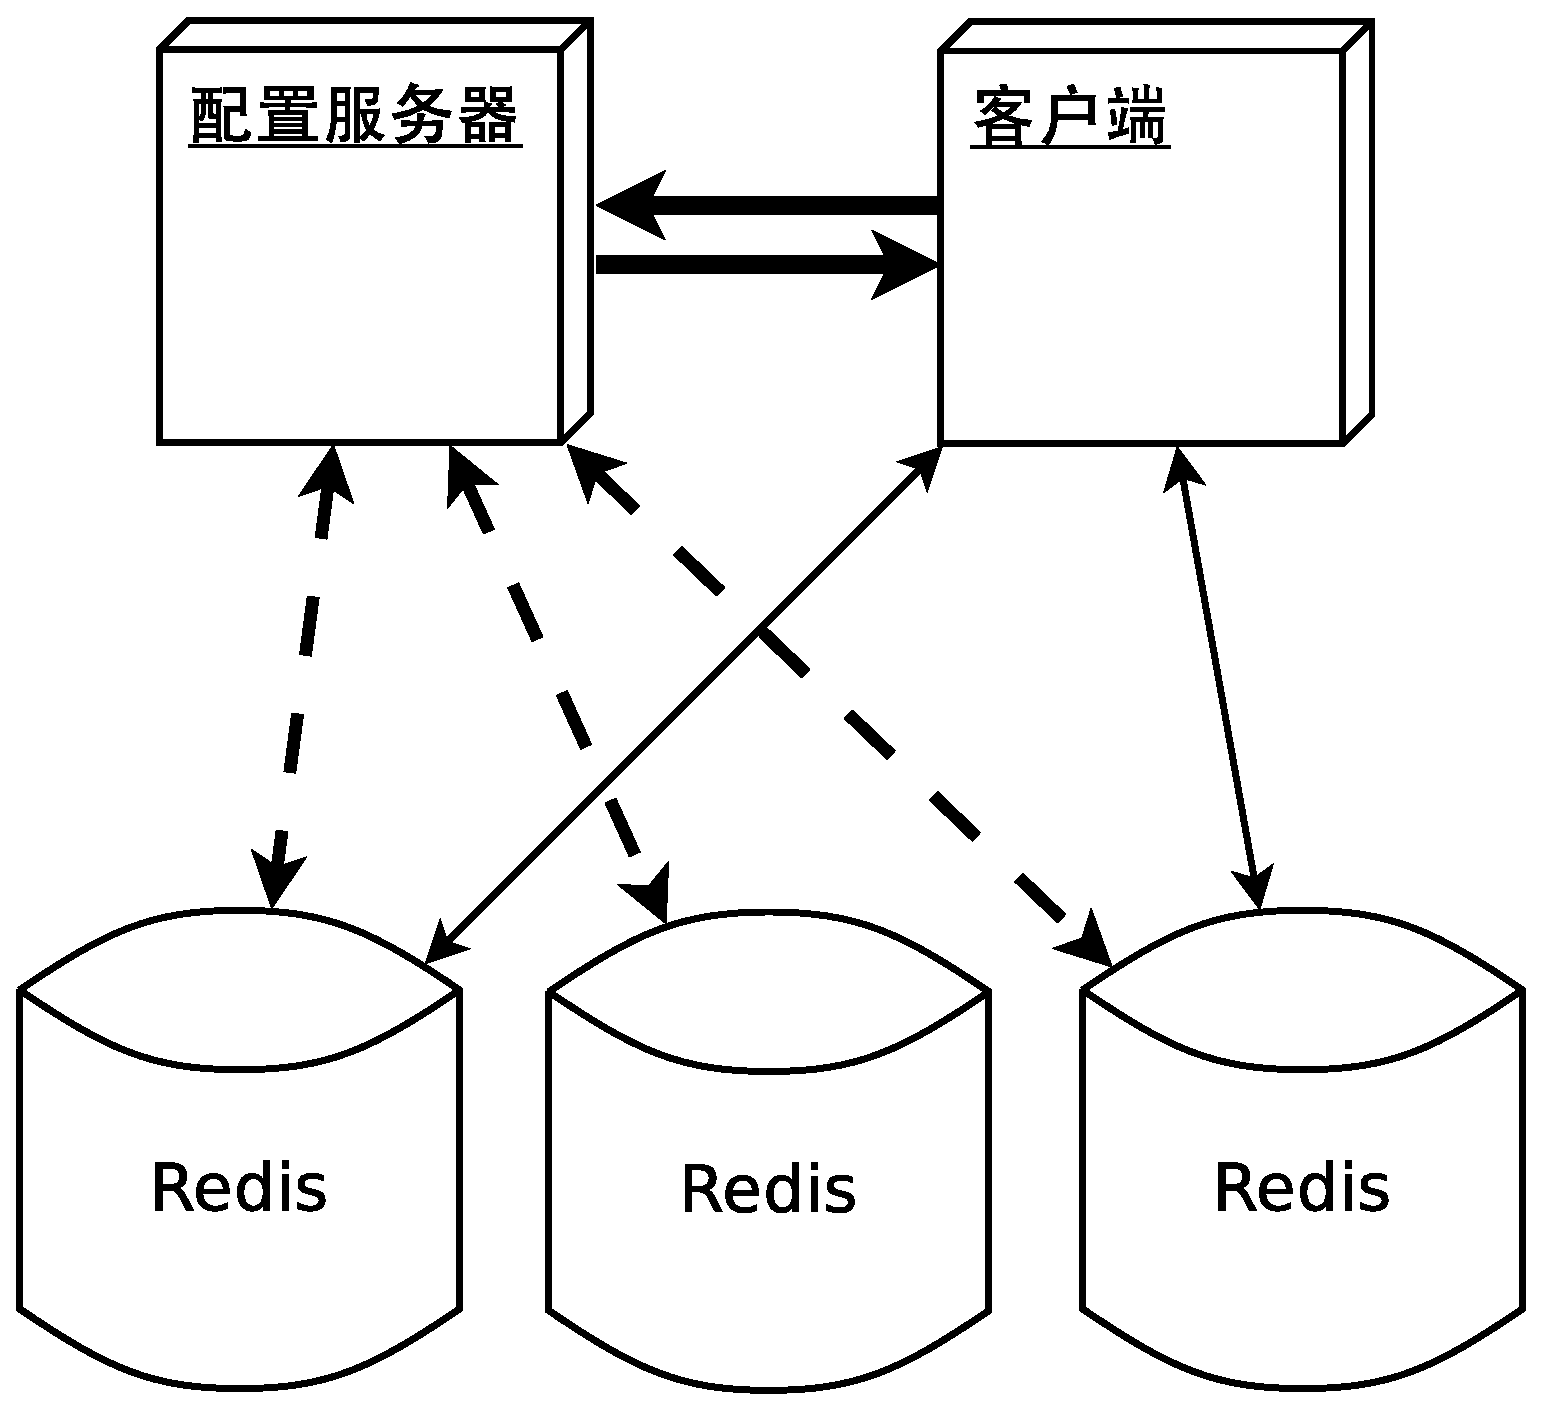
\includegraphics[width=0.8\linewidth]{architecture}
  \caption[分布式二级哈希表系统架构]{分布式二级哈希表系统架构。服务器集群中每
  个存储节点上运行一个Redis服务器进程。集群中设置一台配置服务器,与各节点进行
  心跳通信(虚线箭头),实现一致性哈希。上层应用嵌入客户端库代码,调用其中提供
  的接口函数,首先通过远程过程调用(粗实线箭头)从配置服务器获取某个bucketID对
  应的一系列存储服务器的地址,再遵照协议与这些服务器上的Redis进程进行socket通
  信(细实线箭头),完成相应操作。}
  \label{figure:architecture}
\end{figure}

在存储服务器集群中的每个结点上,都运行着一个Redis存储服务器进程。Redis是一个开
源本地哈希表项目。与一般的哈希表不同,Redis的值类型除了可以是一般的字符串,还
可以是列表、集合甚至哈希。所以Redis实际上已经解决了本地二级哈希的问题。Redis的
另一个优点是它在应用层实现了一个虚拟存储层,将所有数据存于内存和应用层虚存中大
大提高了系统运行效率。同时,Redis是基于日志的事务型存储系统,保证了操作的原子
性,并具备一定的容错能力。有关Redis的更多细节我将在第\ref{section:redis}节做进
一步介绍。

集群中有一台特殊的配置服务器,通过与集群中其他的存储节点进行心跳通信,来确定当
前有哪些机器在正常运行。当前系统不区分不同的故障类型,一概认为该服务器发生了永
久性错误,之后的操作不再涉及该服务器。由于数据有多份副本,不会发生信息丢失。关
于故障处理的更多细节参见第\ref{section:fault}节。配置服务器的另一个功能是实现
了一致性哈希,对于某个特定的目标数据,根据它的bucketID,配置服务器负责指定多个
服务器结点存放该数据,并维护该信息,从而实现了数据的分配和备份。在第
\ref{subsection:consistent}小节我将详细介绍一致性哈希算法。

分布式二级哈希表提供了一个客户端库,里面包含第\ref{section:api}节罗列的接口函
数供上层应用调用,上层应用需要嵌入客户端库代码。当上层应用发起请求时,客户端首
先通过远程过程调用
\footnote{http://en.wikipedia.org/wiki/Remote\_procedure\_call}从配置服务器获
取存放着该数据的多台目标服务器的IP地址,然后按照Redis规定的协议,通过socket通
信\footnote{http://en.wikipedia.org/wiki/Computer\_network\_programming}同时向
这些目标服务器发起请求并接收应答。为了提高系统的运行效率,客户端还做了多项优
化,并且通过线程池实现了异步请求,详见第\ref{section:client}节。

分布式哈希表的架构设计与主流分布式存储系统有很多相似之处,其优点显而易见。
\begin{enumerate}
  \item 数据被分配到多台存储服务器之上,包含多个副本,数据的分配和备份采用一致
  性哈希算法。系统中包含的单个存储单元越多,单个存储单元的容量越大,系统的总存
  储容量就越大。数据分别存放在多台存储服务器上,提升了系统的运行效率。单个存储
  单元的硬盘读写速率和网络带宽是有一个上限,如果客户端能够同时与多台服务器进行
  数据通信,便提高了单位时间内的数据交换速率,使得系统的总体运行效率大大提升。
  另一方面,将数据分配在多台服务器之上,降低了单个存储结点发生错误导致的数据损
  失,增强了系统的容错性。此外,由于系统对数据进行了备份,在不同的存储结点上保
  留了多个副本,即便某个存储节点由于发生了灾难性的故障导致数据永久丢失,系统仍
  可以通过该数据在其他正常运转的服务器上的副本将该数据恢复,正常运转。这大大增
  强了系统的容错能力。一致性哈希算法作为经典的数据分配算法,被很多著名的分布式
  存储系统所采用。\cite{hastorun2007dynamo}由于已知分布式二级哈希表的集群规模
  在几十台服务器左右,机器故障并不会频繁发生,当期的系统实现只保证了数据备份,
  并不支持存储结点动态加入和离开集群。但是一致性哈希算法自诞生之日起,受到青睐
  的原因之一在于它很好的支持了系统中存储结点的动态变化,所以分布式二级哈希表具
  备实现该功能的潜能。事实上,只要在当前系统上添加一个后台数据迁移模块,即可实
  现存储节点的动态添加和移除功能。
  \item 集群中有一台特殊的配置服务器,监控集群中所有存储结点是否运转正常,并实
  现一致性哈希算法。配置服务器与集群中各存储结点进行心跳通信,了解各存储服务器
  的运转情况。相比传输的数据,心跳信息所占用的网络带宽和消耗的系统计算资源基本
  可以忽略不计。因而使用单一的服务器维护控制信息对系统性能造成的影响是微乎其微
  的。另一方面,集中管理控制信息与非集中策略相比,不用考虑信息同步问题,不仅简
  化了系统实现,也方便客户端获得此信息。此外,当前的系统架构设计假设配置服务器
  不会发生系统故障。如果确实需要解决这个问题,只需要再安置一台配置服务器,存储
  控制信息的副本,并定期从主配置服务器获取信息更新。一旦主配置服务器发生系统故
  障,该替补配置服务器立刻接替其工作,继承原配置服务器的属性
  \footnote{如IP地址。},即可实现配置服务器的无缝替换。
  \item 上层应用需要嵌入分布式二级哈希表系统提供的客户端库代码,以调用其中提供
  的接口函数。这种机制在一定程度上影响了系统的易用性,优点是客户端和上层应用之
  间不需要进行网络通信。另一种机制使得上层应用不必嵌入任何系统代码,而是按照系
  统规定的协议与任何一台存储结点或入口服务器通信,再由此机器经过一次路由选择将
  该请求发送至目标服务器,操作完成后再将返回值传回上层应用。缺点是需要附加一次
  网络通信,对网络带宽和操作延迟提出了更高的要求。在
  \onlinecite{hastorun2007dynamo}中详细讨论了两种机制的优劣和适用场合。由于分
  布式二级哈希表在设计之初就本着尽量提高系统运行效率的原则,而其所支撑的上层应
  用目前都是由我们自己设计和实现的工程,所以分布式二级哈希表采用了第一种机制实
  现客户端。
  \item 客户端通过远程过程调用从配置服务器获取存储服务器的IP地址,再与这些存储
  服务器通过Socket通信进行实际的数据传输。在分布式二级哈希表系统中,由于控制信
  息只包含目标存储服务器的IP地址,一次操作需要获取的控制信息只有10字节左右。所
  以尽管整个系统只有一台配置服务器提供控制信息,该服务器依然可以承担相应的负
  担。另一方面,由于实际存储的一份数据最大有1MB,因此实际的数据传输直接在客户
  端和相应的存储服务器之间进行。这种数据分散传输的机制充分利用了各个存储服务器
  的网络带宽和硬盘读写能力,不会由于出现某个瓶颈,而造成整个系统的运行效率降
  低,因而这种设计被很多著名的分布式存储系统所采纳。\cite{ghemawat2003google}
\end{enumerate}

\chapter{原理与实现}\label{chapter:implementation}
分布式二级哈希表是一个偏向工程的项目,涉及到的大多是已经发展成熟的技术,是对分
布式领域一些经典算法的综合。但是分布式二级哈希表对系统的运行效率要求很高,因此
要求在实现细节上不能有瑕疵。本章是论文中篇幅最大的一章,一方面详细阐述了分布式
二级哈希表用到的经典技术的原理,另一方面也深入说明系统的实现细节。

对于像分布式二级哈希表这样并不复杂的系统,在实现时仍然体现了模块化的思想,整个
系统是由一系列模块搭建而成的。每个模块完成特定的功能,基本独立,但是在实现时也
要考虑模块之间的协作关系。这些模块有些是由我独立实现的,有些在实现时参考了别人
的代码,有些将别人的代码加以修改后移植到系统里来,有些则直接使用了别人的代码。
所有的引用和参考都基于开源代码,并且符合作者的协议和使用条款。

分布式二级哈希表的所有模块都用标准C语言写成。相比与其他的脚本语言或者面向对象
编程语言,C语言有着更高的执行效率。C语言的灵活度比较高,对于像分布式二级哈希表
这样对系统执行效率要求颇高的工程,用C语言开发有更大的优化自由度。由于C++语言可
以兼容C语言,但反之不行,所以C语言有更高的可移植性。由于存储服务器上运行的都是
Linux系统,C语言无疑是最佳的选择,所以我决定选用标准C语言实现分布式二级哈希表
的全部开发。另一方面,相比C++语言和其他面向对象编程语言,C语言的标准库和第三方
库都不够丰富,这也迫使我自己实现了像线程池这样的模块,反而锻炼了自己的编程能
力。

下面我将分模块详细阐述每一部分的原理和实现细节。

\section{配置服务器}
配置服务器是整个分布式二级哈希表的核心。它通过与集群中每一个存储服务器进行心跳
通信,掌控集群中所有结点的运转情况。配置服务器实现了一致性哈希算法,负责决定数
据如何在存储结点间进行分配和备份。当上层应用调用系统的接口函数时,客户端首先通
过远程过程调用,从配置服务器获取目标数据所有副本所处服务器的IP地址。在当前的系
统设计中,由于数据已经有多份备份,并且机器故障发生概率很低,所以配置服务器忽略
可能发生的单个结点故障。如果希望配置服务器能够解决存储结点动态加入和离开集群的
情况,需要在当前的系统实现上添加数据迁移模块。

\subsection{一致性哈希算法}\label{subsection:consistent}
一致性哈希算法自诞生之日起,就因其优雅的设计而备受青睐,并且被众多著名分布式存
储系统所采纳。一致性哈希算法的优势在于,当存储结点动态增多和减少时,需要在结点
间转移的数据量最小。虽然分布式二级表的当前设计并不支持结点的动态加入和移除,但
是为了增强系统的可扩展性,我仍然采用了一致性哈希算法来解决数据分配和备份问题。

下面先介绍一致性哈希算法的原理。将哈希函数作用于数据的索引空间,得到的值域空间
称作\emph{哈希空间}。将哈希空间首尾相接,回绕成一个环状空间,称作
\emph{哈希环},如图\ref{figure:consistent}所示。每一个索引的哈希值在哈希环上有
唯一的一个点与之对应,我们用这个点代表具有这个索引的数据。每一个存储结点被称作
一个\emph{物理结点},使用某个字符串作为其唯一标识,比如IP地址。每一个物理结点
有若干\emph{虚拟结点}与之对应,虚拟结点数一般设定为与物理结点的存储容量成正
比。每一个虚拟节点也有一个唯一的字符串标识,一般通过在其对应物理节点的标识后面
附加结点编号构成。图\ref{figure:consistent}中,画出了两个物理结点,其中一个物
理节点画出了两个虚拟结点(深灰色),另一个物理结点只画出了一个虚拟结点(浅灰色
)。将所有虚拟节点的字符串标识求哈希值,结果也是哈希环上的一点,我们用这个点代
表这个虚拟节点对应的物理结点。这样,一个物理结点有几个虚拟结点与之对应,哈希环
上就有几个点与这个物理结点对应。由于哈希函数的性质,与某个物理结点对应的那些点
在哈希环上的分布并无规律可循,当物理结点包含足够多的虚拟结点时,这些点可以看作
是随机分布的。后面我们会看到,正是这个性质保证了一致性哈希在结点动态加入和移出
时,数据迁移量最小。
\begin{figure}
  \centering
  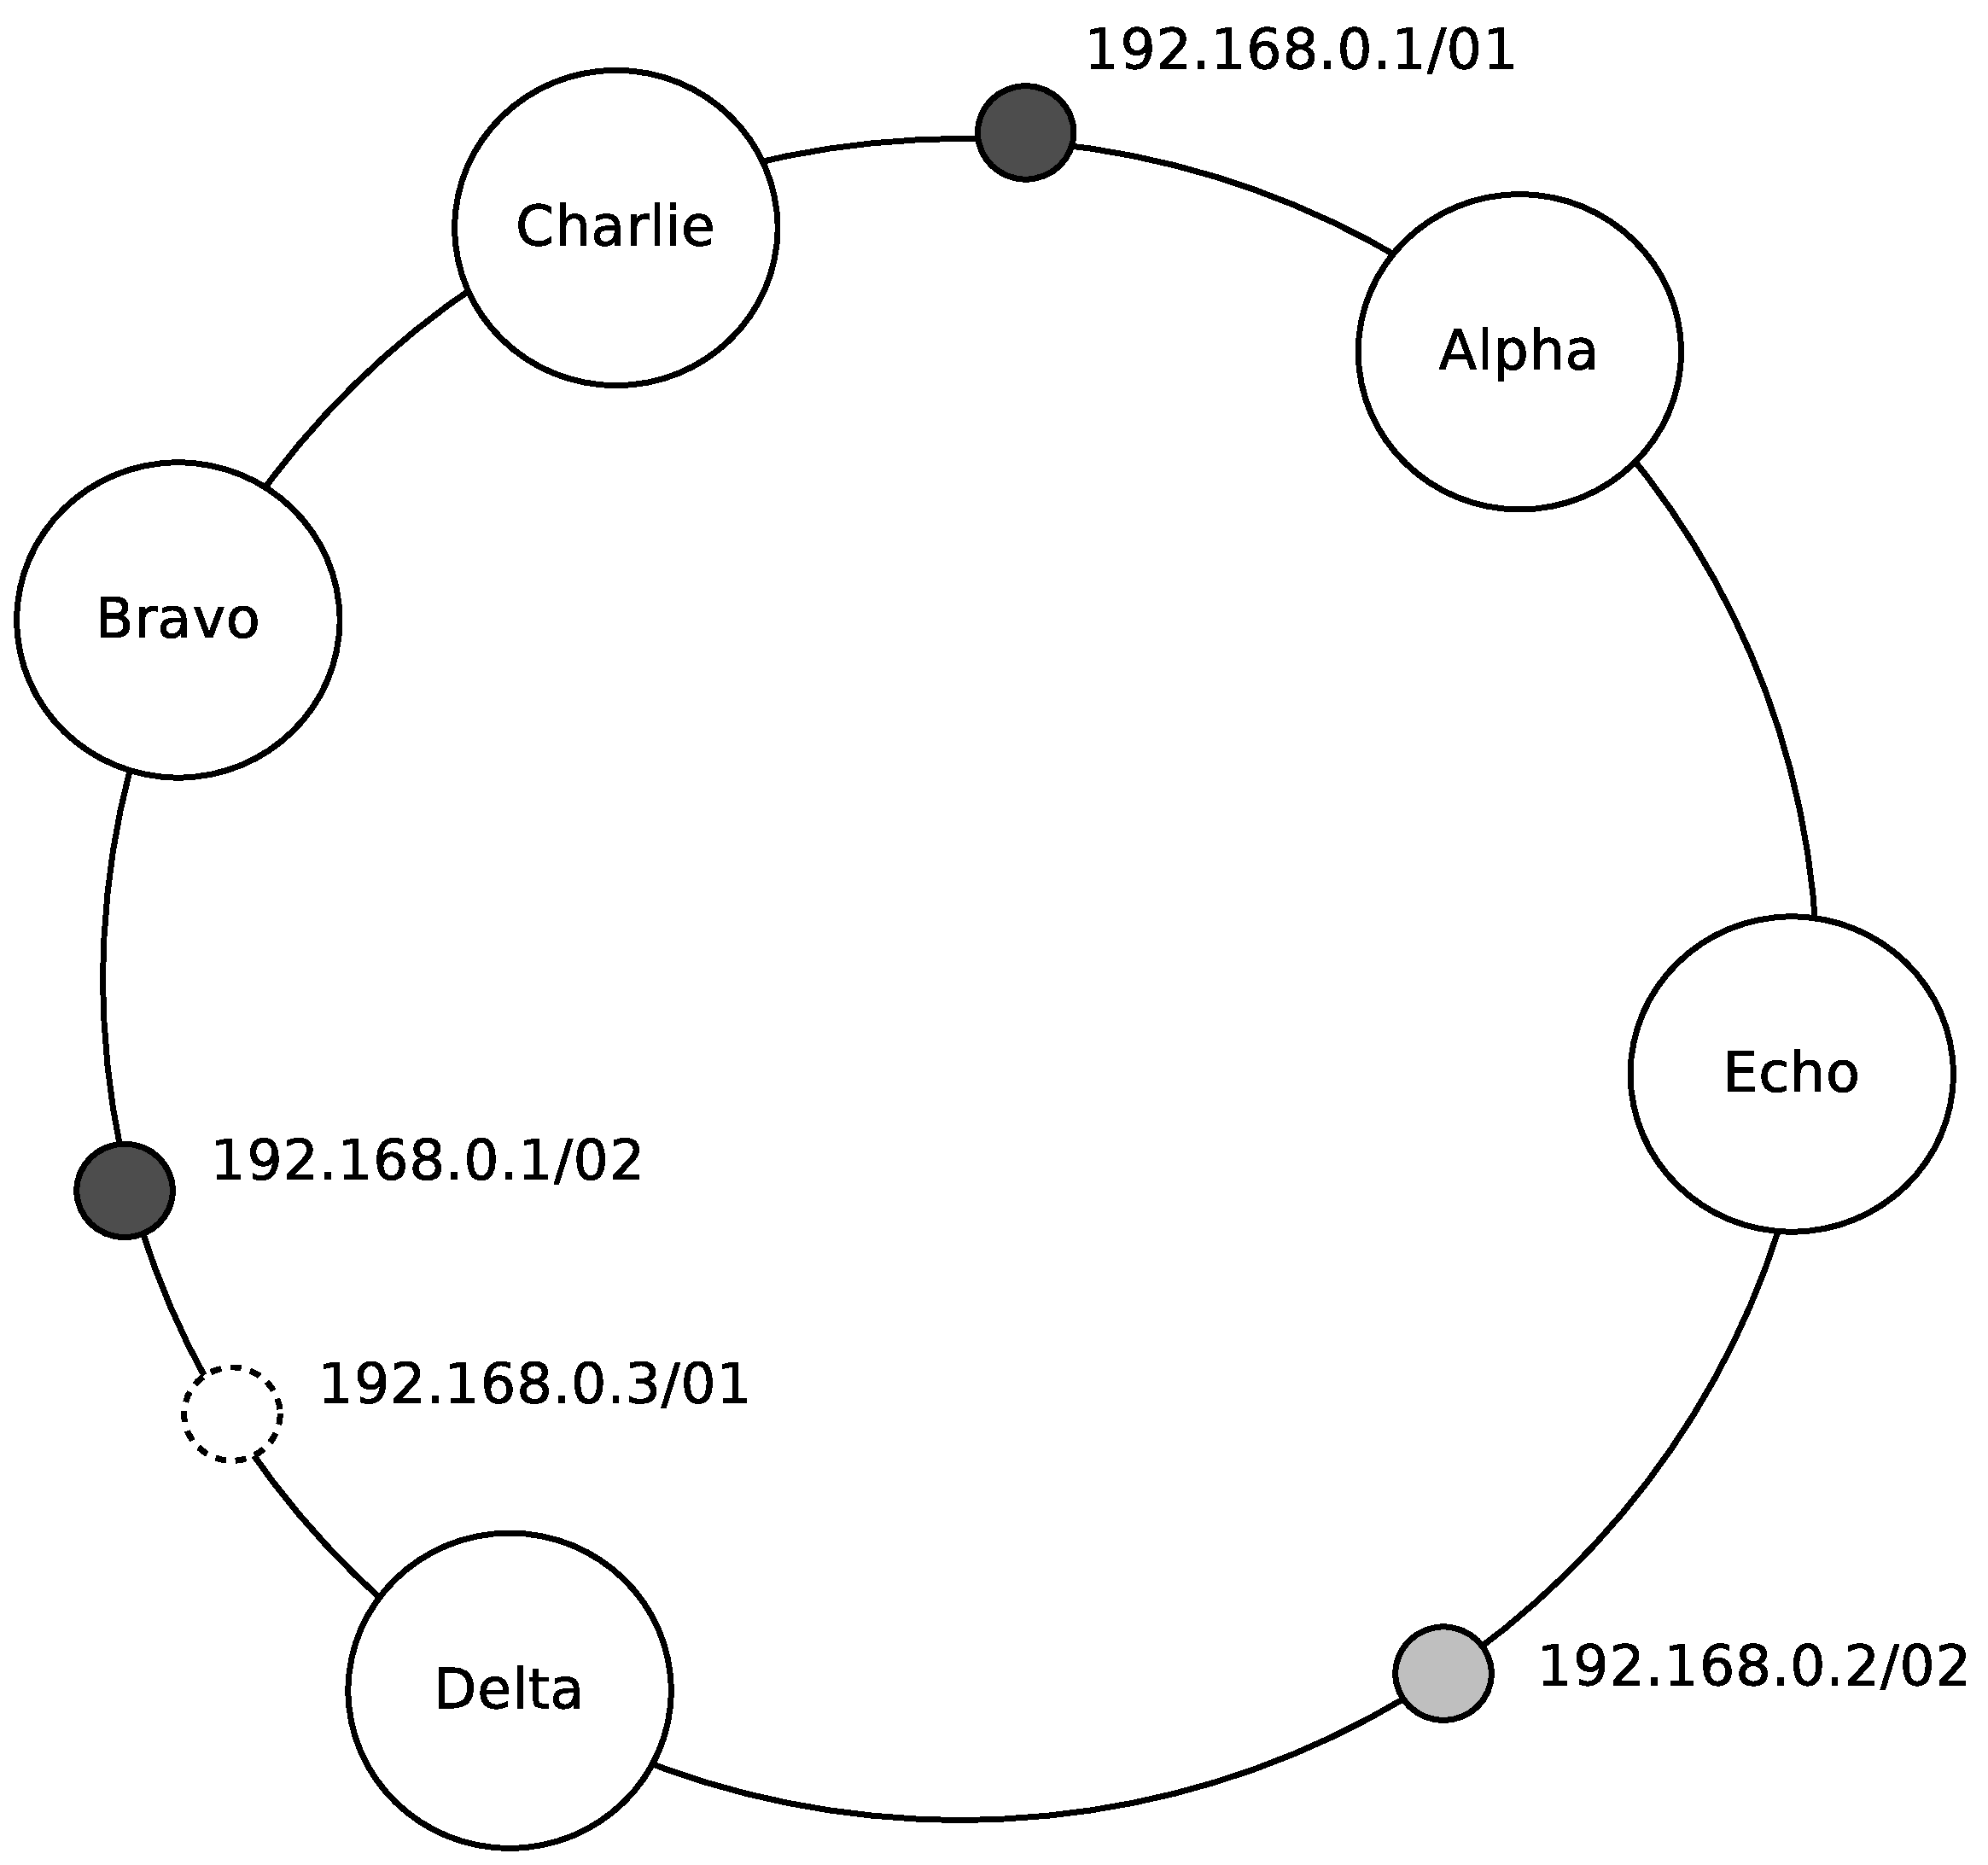
\includegraphics[width=0.8\linewidth]{consistent}
  \caption[一致性哈希算法]{一致性哈希算法。最大的圆环是哈希环。在哈希环上,标
  有字母的大圆代表数据,上面的单词是该数据的索引,图中画出了五个数据。哈希环上
  的小圆代表虚拟结点,旁边标注的字符串是该虚拟结点的标识,同样灰度的小圆对应相
  同的物理结点。系统稳定时有两个物理结点,IP地址为192.168.0.1的物理结点配置了
  两个虚拟结点,用深灰色小圆表示;IP地址为192.168.0.2的物理结点配置了一个虚拟
  结点,用浅灰色小圆表示。对于任何一个数据,其索引的哈希值在哈希环上有唯一的一
  点与之对应。从该点开始,顺着哈希环沿逆时针方向找到M个虚拟结点,这M个结点对应
  的N个不同物理结点即存放该数据的存储服务器,N为数据在系统中的副本数。当系统中
  有新的结点加入,如虚线小圆表示的IP地址为192.168.0.3的存储服务器,假设N等于
  1,需要迁移的数据只有那些索引的哈希值落到从浅灰色虚拟结点到新加入虚拟结点之
  间的劣弧上的数据,这些数据将从深灰色虚拟结点对应的物理结点上移动到新加入的物
  理结点上,即索引值为Delta的数据将从IP地址为192.168.0.1的存储结点上移动到新加
  入的IP地址为192.168.0.3的存储结点上。除此之外,索引的哈希值落在从新加入的虚
  拟结点到浅灰色虚拟结点的优弧上的所有数据都不必做出移动。期望的数据移动量为
  系统中数据总量的(C + 1)分之一,C为结点加入前集群的规模,这也是在保证系统存储
  负载平衡的前提下,任何算法所能达到的数据迁移量下界。此外,一致性哈希算法保证
  了集群中存在结点动态变化时,变化前后系统的存储负载都是均衡的。}
  \label{figure:consistent}
\end{figure}

现在我们有了一个哈希环;对每一个数据的索引求哈希后,在哈希环上都有一点和这个数
据对应;对于集群中的每一台存储服务器,在哈希环上都有若干点与之对应,并且这些点
是随机分布的。在图\ref{figure:consistent}中,最大的圆环是哈希环。在哈希环上,
标有字母的大圆代表数据,上面的单词是该数据的索引。哈希环上的小圆代表虚拟结点,
旁边标注的字符串是该虚拟结点的唯一标识。同样灰度的小圆对应相同的物理结点。那么
如何决定数据的分配和备份呢?一致性哈希算法规定,对于任何一个数据,将哈希函数作
用在它的索引之上,得到的哈希值在哈希环上有唯一一点与之对应。从该点开始,顺着哈
希环沿逆时针方向会找到M个虚拟结点。如果这M个虚拟结点对应N个不同物理结点(N为数
据在整个系统中的副本数,并且显然N不大于M),那么该数据就应当存放在这N个物理结
点上。在图\ref{figure:consistent}中,假设N等于1,那么索引为Alpha的数据应当存放
在IP地址为192.168.0.2的物理结点上,索引为Bravo的数据应当存放在IP地址为
192.168.0.1的物理结点上;如果N等于2,那么图中画出的所有数据都应当在两台服务器
上各存放一个副本。

另一种决定数据在存储服务器之间分配的方法,在实现上比一致性哈希算法简单。首先对
集群中的C台机器从0到C-1依次编号。对于每一个数据,计算其索引的哈希值。由于数据
在计算机中的最终表示是二进制,所以哈希值也可以当成一个整数来处理。将这个整数除
以C,得到的余数即为N等于1时,应当存储该数据的服务器的编号。对于N大于1的情形,
只需要找到编号不小于该余数的连续N台服务器即可。\footnote{如果超过C-1则从0开始
数}这种\emph{除留余数法}与一致性哈希算法相比,思路更加直观,实现也方便,对于集
群结点固定的系统,不失为一种理想的解决方案。

但是在大型的数据中心里,集群规模一般为几千台甚至更多的服务器,结点故障不是偶尔
发生,而是可能一直存在。这要求有一种算法能够应对结点的动态加入和移出,将这种变
化造成的数据迁移量降至最低。对于除留余数法,假设集群中总数据量为D,当有一个新
存储结点加入原本规模为C的集群,那么需要迁移的数据量由公式\ref{equation:modula}
计算得:
\begin{equation}\label{equation:modula}
(\frac{D}{C} - \frac{D}{C - 1}) * (1 + 2 + \dots + (C - 1)) = \frac{D}{2}
\end{equation}
也就是说,当有一个结点动态加入集群时,平均有一半的数据要从原存储服务器移动到另
一台服务器。结点移出集群是加入的逆过程,所有当有一个结点因为故障而不再正常运转
时,平均有一半的数据将发生转移。当结点故障异常频繁时,这种数据迁移规模将耗费大
量的网络带宽和硬盘读写能力,对分布式存储系统将是一个极大的负担。

再回到一致性哈希算法。假设系统稳定后有一个新的存储服务器加入了集群,并且它设置
了一个虚拟结点,如图\ref{figure:consistent}中虚线小圆所示。当N等于1时,需要迁
移的数据只有那些索引的哈希值落到从浅灰色虚拟结点到新加入虚拟结点之间的劣弧上的
数据,这些数据将从深灰色虚拟结点对应的物理结点上移动到新加入的物理结点上,即索
引值为Delta的数据将从IP地址为192.168.0.1的存储结点上移动到新加入的IP地址为
192.168.0.3的存储结点上。除此之外,索引的哈希值落在从新加入的虚拟结点到浅灰色
虚拟结点的优弧上的所有数据都不必做出移动。当N大于1时,情况与之类似,请读者以图
\ref{figure:consistent}为例自行判断哪些数据应该做出移动。那么系统中需要移动的
数据总量是多少呢?考虑结点加入的逆过程,即有一个结点离开集群,需要移动的所有数
据就是这个结点原先负责存储的所有数据。由于每个物理结点对应很多的虚拟结点,而这
些虚拟结点又是随机分布的,因此在结点离开集群之前,数据在集群中的分布是近似平均
的。也就是说,规模为C的集群,一个结点动态离开带来的数据迁移量是$\frac{D}{C}$,
一个结点动态加入造成的数据迁移量是$\frac{D}{C + 1}$。显然这两个数值是在保证系
统存储负载均衡的性质下,数据迁移量的下界。因而当结点动态移入和移出系统时,一致
性哈希算法在数据迁移量方面是最优的算法,并且达到了理论下界。一致性哈希算法的另
一个优点是在集群中结点动态变化时,它仍然保持了系统存储负载均衡的性质。前面已经
分析过,当系统稳定时,一致性哈希算法保证了存储负载均衡。当某个物理结点离开集群
后,原先那些由它某个虚拟结点负责的数据,将被这个虚拟结点按顺时针方向看的下一个
虚拟结点所承担。由于物理结点的所有虚拟结点是随机分布的,那么当一个物理结点对应
足够多的虚拟结点时,这些被选中的虚拟结点将以相同的数目对应全部的物理结点。换句
话说,原先由那个离开的物理结点负责的数据将被平均分成若干份,集群中其余的每个物
理结点将得到相同的份数,所以得到的数据总量也相同。因此,一致性哈希算法保证了集
群中存在结点动态变化时,变化前后系统的存储负载都是均衡的。

分布式二级哈希表的配置服务器实现了一致性哈希算法。开源项目libconhash是一个用标
准C语言写就的,能在Windows和Linux平台下运行的一致性哈希算法实现。但是它不支持
在系统中进行数据备份,并且其中一些功能的实现策略不适合分布式二级哈希表。因此我
在原工程的框架下重写了部分代码,添加了诸多功能,比如使得系统可以支持数据备份,
最终将其成功移植到分布式二级哈希表系统中来。

在分布式二级哈希表中,由于系统设计不予考虑结点动态加入和离开的情形,因此配置服
务器通过读取配置文件获取集群中所有存储服务器的主机名或IP地址。由于集群中各存储
结点是同构的,因此直接设定每个物理结点对应1024个虚拟结点。哈希函数选用128位MD5
哈希\cite{rivest1992rfc1321},保证了虚拟结点在哈希环上的随机分布性质。

实现一致性哈希的另一个关键点是如何在哈希环上快速找到顺时针方向下一个虚拟结点。
由于C语言的标准库中不具有像Java语言中HashMap那样的数据结构可以直接调用实现此功
能的接口函数,在分布式二级哈希表中,这个问题通过自己实现了一棵红黑树
\footnote{http://en.wikipedia.org/wiki/Red-black\_tree}来解决。红黑树是一种平
衡二叉搜索树,它具有以下性质:
\begin{enumerate}
  \item 结点被涂以红色或者黑色。
  \item 根结点被涂以黑色。
  \item 所有叶结点被涂以黑色。
  \item 所有红色结点的左右子结点都被涂以黑色。
  \item 给定一个结点,从这个结点开始到它任何一个后代叶结点的所有路径包含相同数
  目的黑色结点。
\end{enumerate}
这些性质保证了红黑树是一棵基本平衡的二叉树,在它上面进行搜索的最差时间复杂度为
O(log(N)),其中N为红黑树中结点的个数。在分布式二级哈希表中,所有的虚拟结点都有
一个在红黑树中的叶子结点与之对应,排序依据就是这个虚拟结点的标识字符串的MD5
值。当我们需要查看一个某个数据存储在哪些物理结点上时,就把这个数据的索引取MD5
值,再拿这个值在红黑树中去搜索,找到第一个哈希值不小于这个值的虚拟结点,再从这
个虚拟结点的哈希值开始,往后找N - 1个哈希值严格增大,并且对应不同物理结点的虚
拟结点。如果在这个过程中需要找比某个值大的虚拟结点,但是这个值比红黑树中最大的
哈希值还大,那么直接返回哈希值最小的那个虚拟结点。给定索引确定数据所在存储服务
器的IP地址的函数伪代码如下:
\begin{code}
  FUNC getIpsByKey(IN string key, IN int N, OUT IP[] ips)
  {
    GLOBE RBTREE rbtree;
    VAR VNODE vnode, start;

    vnode = rbtree.geq( MD5(key) );
    ips[0] = vnode.node.ip;
    start = vnode;
    for i from 1 to (N - 1)
    {
1:    vnode = rbtree.ge( vnode.hash );
      if ( vnode == start ) ERROR;
      for j from 0 to i - 1
      {
        if ( ips[j] == vnode.node.ip ) goto 1;
      }
      ips[i] = vnode.node.ip;
    }
  }
\end{code}
前面我们说到在红黑树中搜索的时间复杂度为O(log(N)),其中N为树中结点总个数。在分
布式二级哈希表的一致性哈希实现中,红黑树中的结点数就是系统中虚拟结点的总数。在
第\ref{section:assumption}节中的一个假设是系统的典型规模为50台存储服务器,按照
上文提到的每个物理结点配置1024个虚拟结点计算,一次查询需要花费的时间规模与处理
器进行16次运算相当,因此用红黑树实现一致性哈希具有很高的查询效率。

此外,之前在原理介绍中提到的数据索引,在分布式二级哈希表的实现中,指的是blob的
bucketID。也就是说,同一个桶中的blob将存储在相同的服务器上。一致性哈希算法对于
数据的分配粒度是相对于桶的,它不能区分同一个桶中不同的blob。在这种情况下,集群
的存储负载平衡是由另一个假设保证的。即我们假设单个blob较小,但是blob和桶的个数
很多。如果我们将桶中所有blob的大小求和作为桶的大小,那么虽然桶的大小可能差异很
大,但是由于每个物理结点都存储了很多的桶,而且这些桶是随机分配的,那么当桶的数
目足够多时,每个物理结点的总存储量是近似相同的。

\subsection{远程过程调用}
除了一致性哈希算法,配置服务还包含另一个重要模块,即远程过程调用模块。在分布式
二级哈希表中,客户端通过远程过程调用从配置服务器获取某个数据所在的目标存储服务
器的IP地址。

远程过程调用是一种客户端和服务器交互的技术,它使得客户端程序可以调用执行在远端
服务器上的一段程序,而调用方法就好像在执行本地的函数一样,不必客户端和服务器的
网络交互,以及其他实现细节。分布式二级哈希表采用ONC RPC
\footnote{http://en.wikipedia.org/wiki/ONC\_RPC}标准规定的远程过程调用协议,代
码执行流如图\ref{figure:oncrpc}所示。客户端执行callrpc系统调用,并将参数按照本
地函数调用的方式压栈。callrpc从中提取出目标服务器例程的信息,并将该例程需要的
参数按照事先定义的方式打包,然后通过TCP或UDP协议将参数发送至指定服务器。目标服
务器事先已经注册了一段例程,并监听ONC RPC使用的默认端口111。一旦收到客户端发来
的打包数据,按照事先定义的方式从中提取出参数,并传递给服务器例程。接着服务器例
程在用户态执行,执行完毕后,进入内核态,由操作系统将返回值按照事先约定的方式打
包,再依照相同的传输层协议,通过刚才建立的连接,将打包后的返回值传回客户端。至
此,此次远程过程调用服务器端的工作完成,服务器端准备应答下一个请求。客户端收到
服务器发送来的打包数据,按照事先约定的方式从中提取出返回值。然后callrpc系统调
用返回,将远程过程调用的返回值传递给用户态的客户端主程序,本次远程过程调用执行
完毕。
\begin{figure}
  \centering
  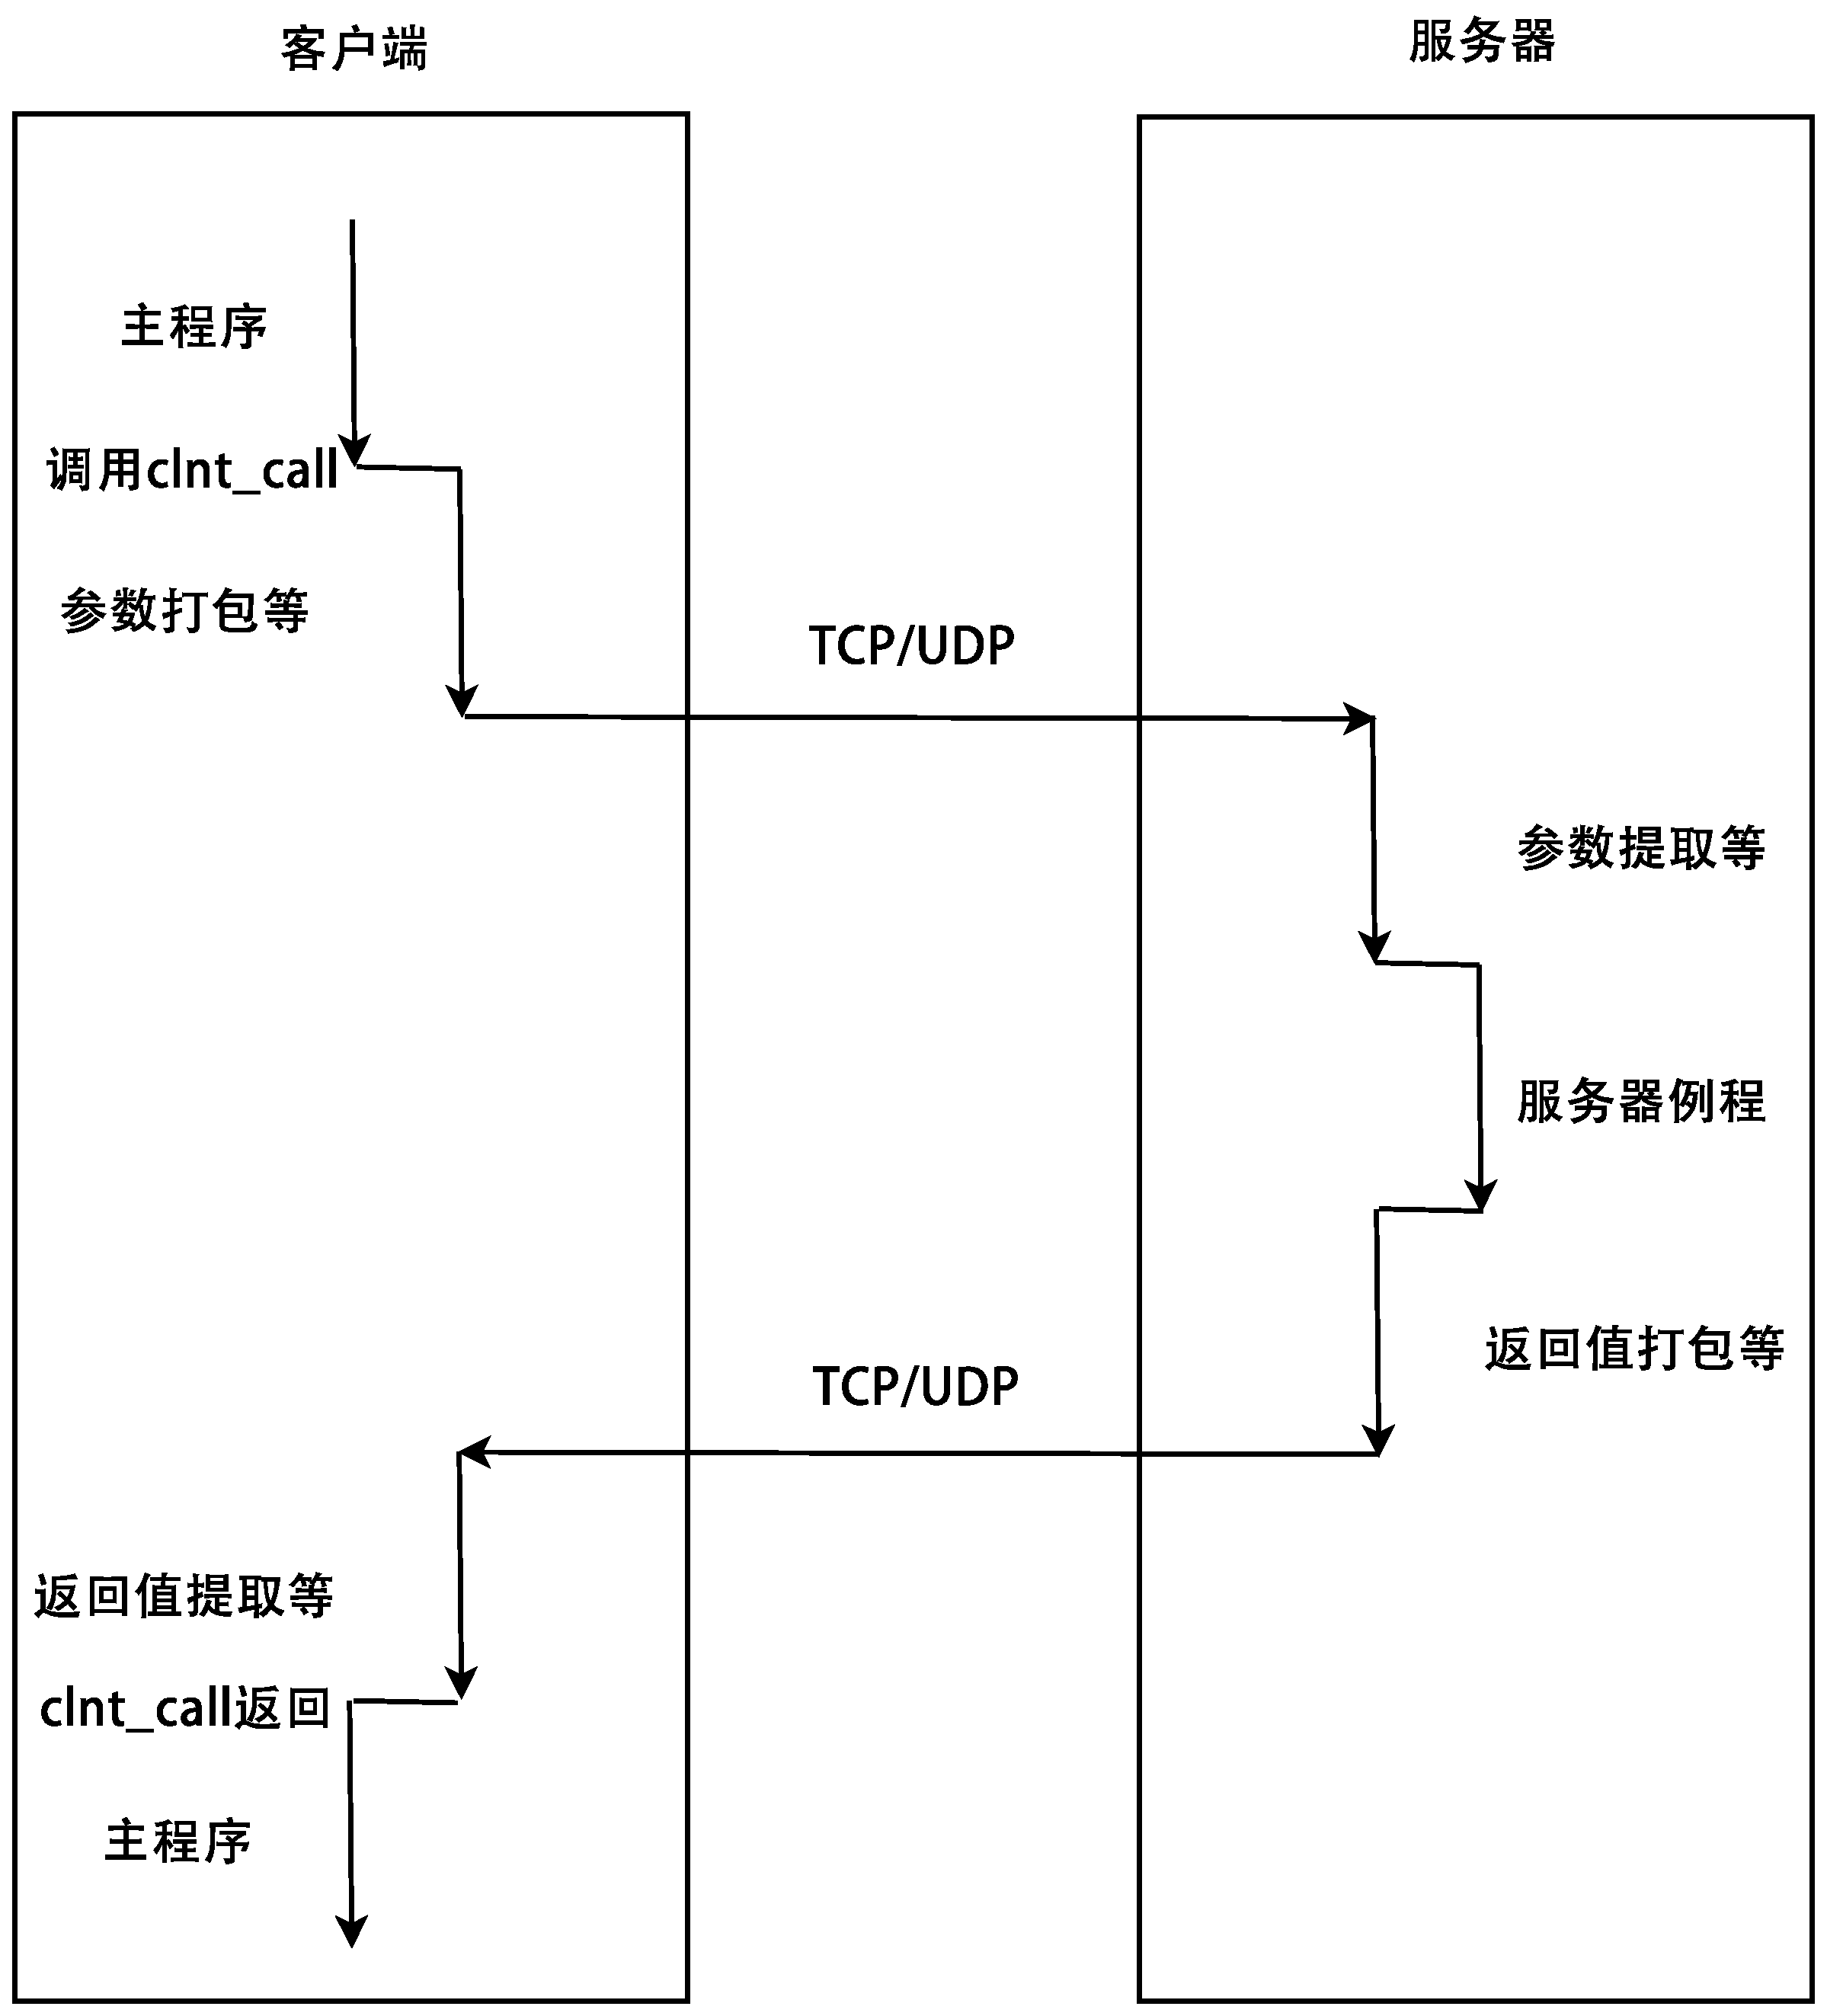
\includegraphics[width=1.0\linewidth]{oncrpc}
  \caption[ONC RPC代码执行流]{ONC RPC代码执行流。客户端用户态主程序执行
  callrpc系统调用。callrpc将服务器目标例程需要的参数按照事先定义的方式打包,然
  后通过TCP或UDP协议将打包数据发送至指定服务器。目标服务器事先已经注册了一段例
  程,并监听ONC RPC使用的默认端口111。收到客户端发来的打包数据后按照事先定义的
  方式从中提取出参数,并传递给用户态服务器例程。服务器例程执行完毕后,进入内核
  态,由操作系统将返回值按照事先约定的方式打包,再通过刚才建立的连接将打包后的
  返回值传回客户端。至此,此次远程过程调用服务器端工作完成,端准备应答下一个请
  求。客户端收到服务器发送来的数据,按照事先约定的方式从中提取返回值。然后
  callrpc返回,将远程过程调用的返回值传递给用户态的客户端主程序,本次远程过程
  调用执行完毕。}
  \label{figure:oncrpc}
\end{figure}

远程过程调用这种客户端和服务器的交互机制,简化了程序员的变成,其中,参数和返回
值的打包,数据在客户端和服务器之间的可靠性传输等工作均由系统来实现。但是,上述
代码执行流程对于纯粹写应用的程序员仍然略显复杂,比如,程序员需要\emph{告知}系
桶如何对数据进行打包和提取,需要初始化网络参数等。为了进一步简化程序员编程,使
程序员将主要精力放在将要实现的功能上,而不是远程过程调用本身的实现上,编程工具
rpcgen\footnote{http://en.wikipedia.org/wiki/Rpcgen}应运而生。程序员只需要书写
一个简单的配置文件,声明服务器例程的原型,以及各参数和返回值的数据结构,rpcgen
就能据此产生出服务器和客户端将要用到的全部C代码。程序员只需要在服务器端例程的
框架里填入具体实现,再将客户端代码和服务器端代码分别编译,便实现了远程过程调
用。比如,在分布式二级哈希表中,客户端通过远程过程调用,给定一个索引,从配置服
务器得到具备这个索引的数据所在的存储服务器的IP地址。那么rpcgen的配置文件
cfgsrv.x内容非常简单:
\begin{code}
typedef u_int ips<>;

program CFGSRVPROG {
  version CFGSRVVERS {
    ips GET_HOSTS_BY_KEY(string) = 1;
  } = 1;
} = 1;
\end{code}
其中指定了服务器端例程的原型。参数只有一个,即字符串类型的索引值。返回值是无符
号类型整数的可变长度数组,其中每个元素是一个目标存储服务器的IP地址。rpcgen据此
生成了四个文件:
\begin{enumerate}
  \item cfgsrv.h: 基本的声明文件。编译客户端和服务器端程序时都需要引入此头文
  件。
  \item cfgsvr\_clnt.c: 客户端辅助文件,以实现远程过程调用机制,其中只定义了一
  个函数get\_hosts\_by\_key\_1。客户端主程序调用这个本地函数,就能从配置服务器
  获取目标存储服务器的IP地址。
  \item cfgsrv\_svc.c: 服务器端辅助文件,以实现远程过程调用机制。
  \item cfgsrv\_xdr.c: 服务器端例程的参数和返回值打包程序。
\end{enumerate}
为了完成远程过程调用机制,服务器端还需要实现cfgsrv.h中声明的
get\_hosts\_by\_key\_1和get\_hosts\_by\_key\_1\_svc两个函数。其中第一个函数是
服务器端真正完成通过索引获取目标存储服务器IP地址的例程,可以调用第
\ref{subsection:consistent}小节介绍的一致性哈希算法的实现函数。第二个函数只是
对第一个函数的包装。之后通过rpcgen -m命令可以得到服务器端初始化远程过程调用的
代码。至此,将上述文件合理编译,即可得到实现了远程过程调用的服务器和客户端模
块。

远程过程调用简化了客户端和服务器端实现通信的机制。如果不使用远程过程调用,一种
实现方式是直接在客户端和服务器端建立TCP/UDP连接,再按照自定义的协议传送数据。
在第\ref{section:assumption}实验假设中提到分布式二级哈希表平均每台服务器每秒处
理的请求数不小于50,平均响应时间为百毫秒数量级,这说明客户端一直会发起大量的请
求。如果每一个请求完成之后都关闭socket连接,下个请求到来时再重新建立连接,那么
创建socket和回收资源的系统开销将会非常大,严重影响系统运行性能。这要求每个客户
端和配置服务器的socket连接一直持续,直到客户端程序全部运行结束。基于这个前提,
由于要保证系统的平均响应时间和吞吐量,请求必须设定为异步的,而不能像同步系统那
样将请求放置在一个队列里,在上一个请求结束之后再处理下一个请求。因此,请求的返
回顺序可能和发起顺序不同,客户端可能先收到后发出的请求的返回值,再收到先发出的
请求的返回值。在同一个socket连接中,客户端需要为每个请求附上一个唯一的流水号,
服务器则要为返回值贴上相同的流水号。另一方面,在编程实现上,异步请求也较同步请
求更为复杂,容易出错且不易调试。如果维护返回值和请求的对应关系,以及请求的异步
化都由远程过程调用的框架来完成,那么对于程序员来说,客户端的每次请求就是对本地
函数的一次调用,不必过多考虑上述实现细节。

\section{客户端}\label{section:client}
在第\ref{chapter:architecture}章中曾介绍过,分布式二级哈希表中的客户端是一个独
立的模块,是分布式二级哈希表的一个函数库,上层应用需要将这些代码编译到可执行文
件中去。客户端直接从配置服务器拿到目标存储服务器的IP地址,再与这些服务器进行通
信,执行操作,并将返回值传递给上层应用。这样,完成一次操作总共需要进行两次网络
通信。第一次是客户端通过远程过程调用从配置服务器拿到路由信息,第二次是客户端将
请求发送给具体的存储结点,得到返回值。这种决策的缺点是上层应用需要嵌入分布式二
级哈希表的标准C代码,降低了分布式二级哈希表的易用性和通用性。另一种不许要嵌入
系统框架代码的解决方案是,让客户端直接与某一台入口服务器按照某种协议进行通信,
再有这台入口服务器完成客户端的功能。这样入口服务器和客户端之间还要多进行一次网
络通信,势必增加请求的平均响应时间,并且消耗网络带宽。由于分布式二级哈希表更在
意系统的运行效率,而且上层应用是由我们自己搭建的,因此最终我选用了第一种方案来
实现客户端。

客户端采用了分层结构,如图\label{figure:client}所示。
\begin{figure}
  \centering
  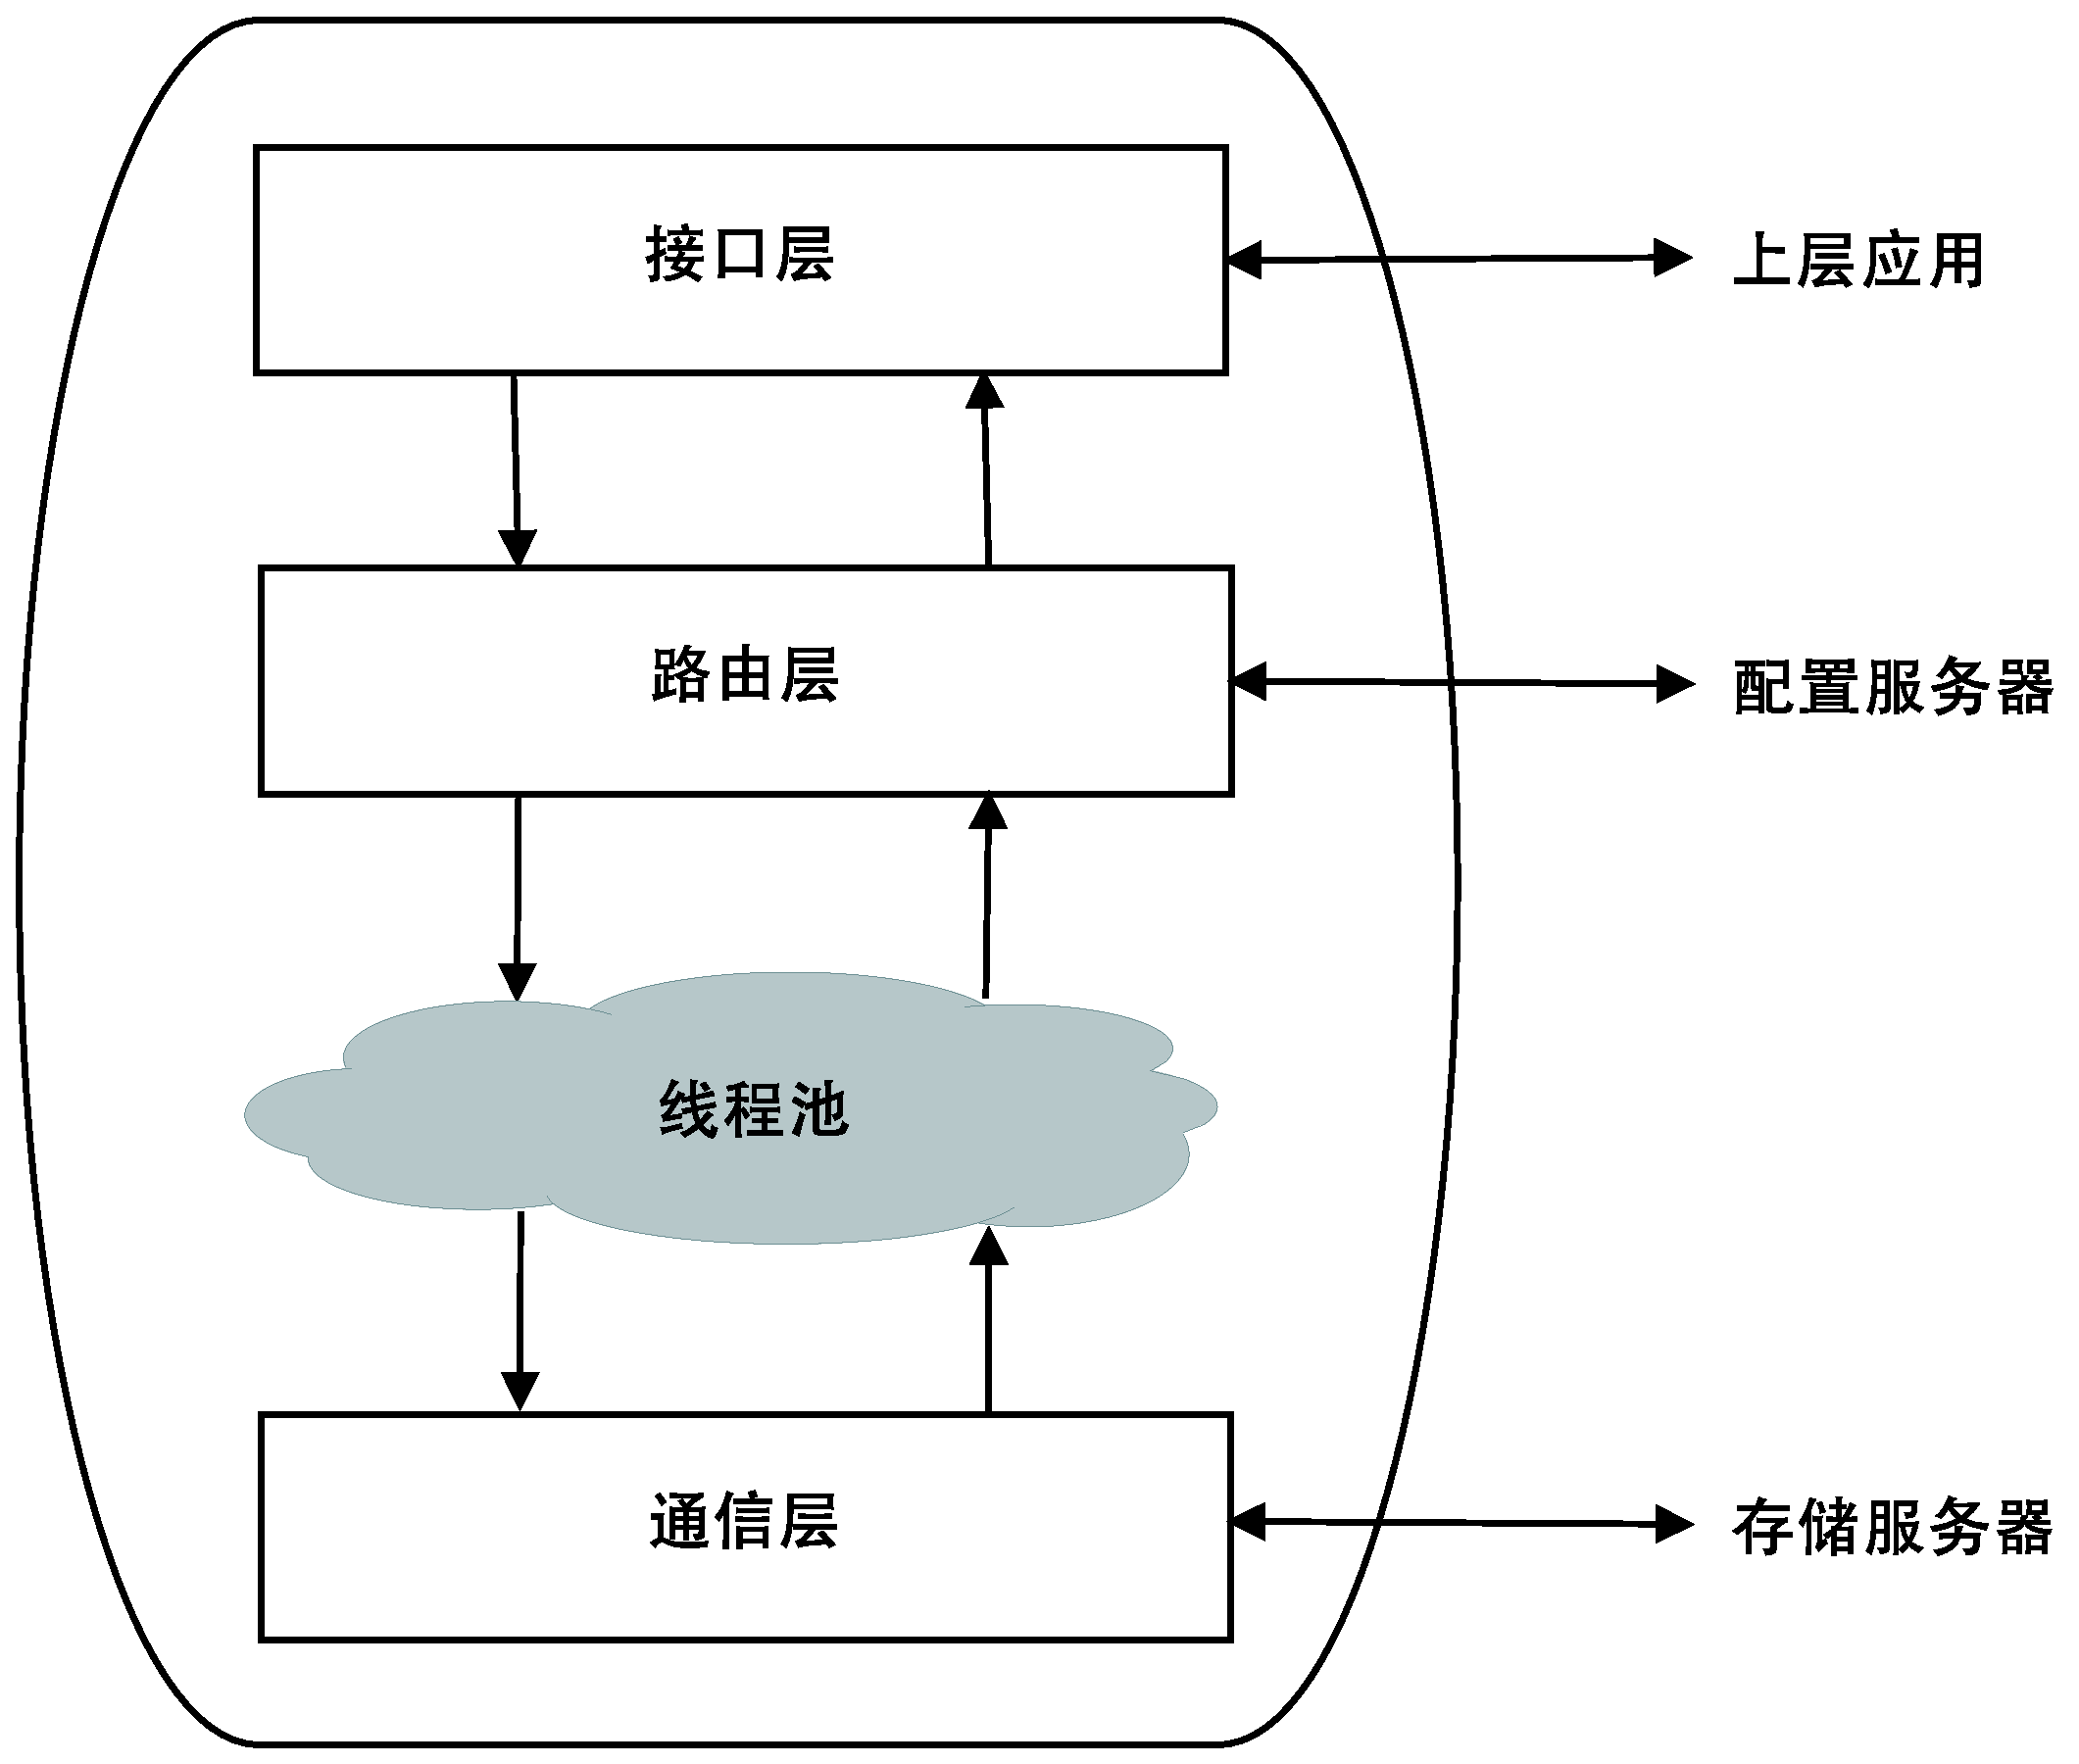
\includegraphics[width=0.8\linewidth]{client}
  \caption[分布式二级哈希表客户端]{分布式二级哈希表客户端。}
  \label{figure:client}
\end{figure}

\section{Redis}\label{section:redis}

\section{容错}\label{section:fault}


\chapter{实验与结果分析}\label{chapter:lab}

\chapter{缺陷与改进方案}\label{chapter:future}


%%% 其它部分
\backmatter

% 本科生要这几个索引,研究生不要。选择性留下。
\makeatletter
\ifthu@bachelor
  % 插图索引
  \listoffigures
  % 表格索引
  \listoftables
  % 公式索引
  \listofequations
\fi
\makeatother


% 参考文献
\bibliographystyle{thubib}
\bibliography{ref/refs}


% 致谢
\begin{ack}
衷心感谢我的导师陈文光教授对我完成毕业设计给予的悉心指导,感谢我的辅导教师陈康
副教授对我的热心辅导与帮助。

感谢清华大学计算机科学与技术系高性能所集群计算组实验室的各位学长学姐,长期以来
对我提供了各方面的热心帮助,耐心地为我答疑解惑,使我能够顺利完成毕业设计。

在写作论文的过程中,我使用了\LaTeX 工具。开源模板\thuthesis 大大简化了写作论文
的工作量,特此感谢。
\end{ack}


% 附录
\begin{appendix}
\chapter{外文资料的的调研阅读报告}

\begin{center}
A Brief Report on Distributed Storage System
\end{center}

\section*{Introduction}
Distributed system is a major topic of current computer science. Among it, a
distributed storage system usually takes advantage of multiple machines to
gain capacity, reliability, availability, while for people who operates data,
it seems that he is facing with a single machine and needn't care about the
whole backend framework.

\section*{Categories}
There are a lot of typical distributed storage systems. Google File System
$^{[1]}$, MooseFS\footnote{http://www.moosefs.org/} and many others are
classified as \emph{distributed file system}. A client can communicate with
the cluster to store and retrieve data much like operating files in a local
file system. Usually, they support full namespace hierarchy and the data is
accessed with a path.

Another category is classified as \emph{distributed database}. The significant
feature of the data stored in a distributed database is that the data is
stored and accessed aligned by \emph{columns} and \emph{rows}. Sometimes, more
strengthful databases also record relationship between data and support
complicated query semantics.

Apart from the two categories mentioned above, a novel kind of distributed
storage system is getting more and more popular. It is not only
light-weighted, as it doesn't support relationship between data or just
supports weak relationship, but also flat, usually because it doesn't support
complicated namespace hierarchy but just a map of key-value pairs. On the
opposite, the system which belongs to this category is usually of high
performance, to be measured by throughput, latency, availability, reliability
and other criteria. Such systems are called \emph{distributed key-value
stores}. Douban's BeansDB
\footnote{http://beansdb.googlecode.com/files/Inside\%20BeansDB.pdf}, Kyoto
Cabinet\footnote{http://fallabs.com/kyotocabinet/kyotoproducts.pdf} from Japan
and many others are all successful distributed key-value stores. As such
storage systems are light-weighted, some systems, like MemcacheDB
\footnote{http://memcachedb.org/memcachedb-guide-1.0.pdf}, decide to put data
in memory or virtual memory to gain performance burst.

\section*{Fundamental Concepts}
Before I summarize existing distributed storage systems, I would like to
explain some fundamental concepts related to distributed system. Without a
clear introduction on these conceptions, it would be impossible to comprehend
the beauty and elegance of architecture designs on famous distributed storage
system.

\subsection*{Replication}
Replication is copies of same data. In distributed system, data is distributed
to many computing and storage machines. Under most cases, data is evenly
stored on different machines. The world will be easy but fragile if we don't
make copy of data. Let's take a closer look at why data backup is necessary
with some simple calculation. If the possibility of failture for a single
machine is $p$, and for simplicity, we assume all the machines are
independently identical, i.e., the possibility of failure for each machine
equals $p$ and a machine never notices whether his buddy is alive or dead.
What is the possibility that a system containing $n$ identical machines goes
down with one or more machine failing to work at some time? Yes, you are
right! It is $1 - (1 - p)^n$. So what does this mean? Although $p$ may be
small, when $n$ gets larger and larger, the result tends to reach 1! Commonly,
a datacenter of companies like Google contains from thousands of to millions
of machines with moderate disks. Disk failures are not rare but a common case.
If the data is not replicated, it would be impossible to ensure the integrity
of data, as recovery of data from a failed disk costs time, computation
resource and network bandwith, yet this is not always possible. Hence making
copies of data is critical in large systems like distributed key-value store.

\subsection*{Consistent Hashing}
Replication of data may not be as simple as it seems at first glance. There
are many tricky technologies behind to provide the correctness of the
replication mechanism, and further the improvement of the performance.
Situation becomes even worse when the system is distributed as we have to make
decision on the choice of machine for different block of data.

Usually, the data is distributed by its key. First, a hash function is needed
to calculate a hash value for the key. The key may be a string or even any
binary stream, while the result of the hash function always falls into a
finite range. The range, called \emph{hash space}, is divided into several
segments, each representing a machine. That machine takes responsibility of
all the data with keys whose hash value is within that range.

Different distributed algorithms vary in their hash functions. A simple
instance could be a distributed system which adopts \emph{Cyclic Redundancy
Check} as its hash function. As we mentioned above, each machine is associated
with a segment in the range of hash value. However, in most cases, this range
is further made up of several sub-segments, called hash slots. Often, hash
slots within a segment are not located adjacently to each other in the hash
space. Note that this is why the algorithm distributes data evenly among
different machines, while the impact of a single machine failure is minimized.

Consistent hashing$^{[4]}$ is a method to distribute data evenly within a
storage cluster, regardless of the specific hashing function employed. If we
concatenate the tail of the hash space to its head, the hash space will rewind
like a ring, called the \emph{hash ring}. We put some nodes on the ring and
the ring is broken up into some arcs. These nodes are called \emph{virtual
nodes}. A physical node is a storage server, which is a collection of same
amount of virtual nodes. The assignment of virtual node to physical one is
random, which means that all the virtual nodes, which belong to the same
physical node, may not be adjacent on hash ring. Different virtual nodes,
which belong to different physical nodes, may not appear on the hash ring in a
round-robin manner. They are just randomly distributed.
    
How to decide which storage server should take responsibility of the data
associated with a specific key? If we don't take data replication into
consideration, the server is the physical node found as follows. We traverse
clockwise from the point on the hash ring representing the hash value of that
key. The physical node, where the first virtual node met like this belongs to,
is the storage machine which is responsible for that data.

When a machine refuses to work any more due to failure, the virtual nodes
associated with it should be taken care by other physical nodes. It is obvious
that each of such virtual nodes should share the same physical node, to which
the next virtual node belongs, counting clockwise. As the virtual nodes
conducted previously by the failed machine are distributed randomly, it is
probably expected that the data handled previously by the failed machine will
be distributed evenly across other active machines. It goes the same when a
new machine joins the cluster.

In the real world, data is replicated into many copies. The data associated
with a single key is stored on several machines, namely N physical nodes.
These machines are determined by tranversing clockwise from the point on the
hash ring representing the hash value of that key. The traversal stops when
the first M virtual nodes belongs to N different physical nodes. These N
physical nodes are the target machines.

\section*{Example Distributed Storage Systems}
In this short article, I'll make a brief summary on several famous distributed
storage system with introductions on their significant features.

\subsection*{Dynamo: Amazon's Highly Available Key-value Store}
I believe the most famous distributed key-value store is Amazon's Dynamo
$^{[2]}$. Although it is neither open source nor
available for organizations outside Amazon to use, it is highly recognized by
scientists and engineers in the area of distributed computing.

Perhaps Dynamo gains popularity mainly because of its elegant design. It is a
perfect example of minimizing system functionality to satisify basic
requirements of application. Dynamo acts as an internal infrastructure for
Amazon's many services, such as the on-line book stores. In most of the
senarios, the service beyond Dynamo has such a requirement that data is highly
writable. Considering this specific requirement, Dynamo is designed at first
day to support high throughput and low latency of write request, while to
sacrifice consistency hence increasing of read request both operation time and
possibility of version conflict, which is tolerable within these services.

\subsection*{Bigtable: A Distributed Storage System for Structured Data}
Bigtable$^{[3]}$ is an outstanding representative of the brand
new \emph{NoSQL}. It differs from traditional database by not supporting
complex relationship between data, yet more flexible. Bigtable is considered
as a multi-dimensional mapping of data. The last dimension is usually
timestamp which means the database records historical snapshots of data. The
database is flexible that dimension names of different data may be different.

\subsection*{Redis: An Open Source, Advanced Key-value Store}
Redis\footnote{http://redis.io/} is an open source key-value store. It beats
other hash tables for its rich type of values, such as binary stream, lists,
sets, sorted sets and even hashes, while still maintaining high performance
because all the data resides in memory. Redis not only performs data
compression but also implements a virtual memory layer in user space to solve
memory shortage. It is also fully journaled to enhance ability of fault
tolerance.

\begin{center}
参考文献
\end{center}
\begin{enumerate}[{[}1{]}]
  \item Ghemawat S, Gobioff H, Leung S. The Google file system. Proceedings of
  ACM SIGOPS Operating Systems Review, volume 37. ACM, 2003. 29–43
  \item Hastorun D, Jampani M, Kakulapati G, et al. Dynamo: amazon’ highly
  available key-value store. Proceedings of In Proc. SOSP. Citeseer, 2007
  \item Chang F, Dean J, Ghemawat S, et al. Bigtable: A distributed storage
  system for structured data. ACM Transactions on Computer Systems (TOCS),
  2008, 26(2):1–26
  \item Karger D, Lehman E, Leighton T, et al. Consistent hashing and random
  trees: Distributed caching protocols for relieving hot spots on the World
  Wide Web. Proceedings of Proceed-ings of the twenty-ninth annual ACM
  symposium on Theory of computing. ACM, 1997. 654–663
\end{enumerate}

\end{appendix}

% 综合论文训练记录表
\begin{figure*}
  \centering
  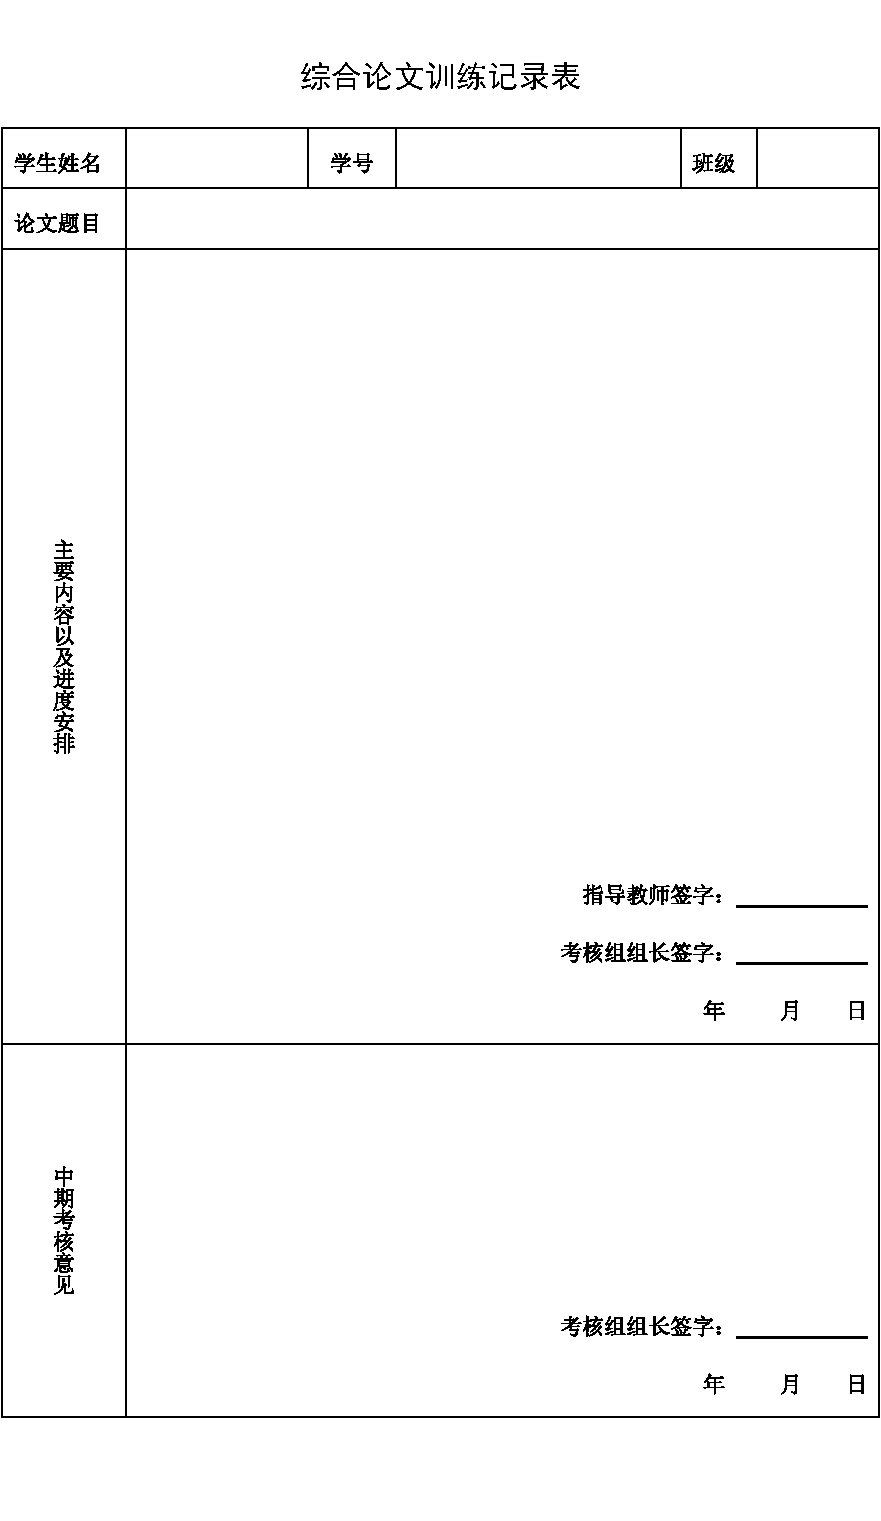
\includegraphics[width=0.95\linewidth]{record1-crop}
\end{figure*}
\begin{figure*}
  \centering
  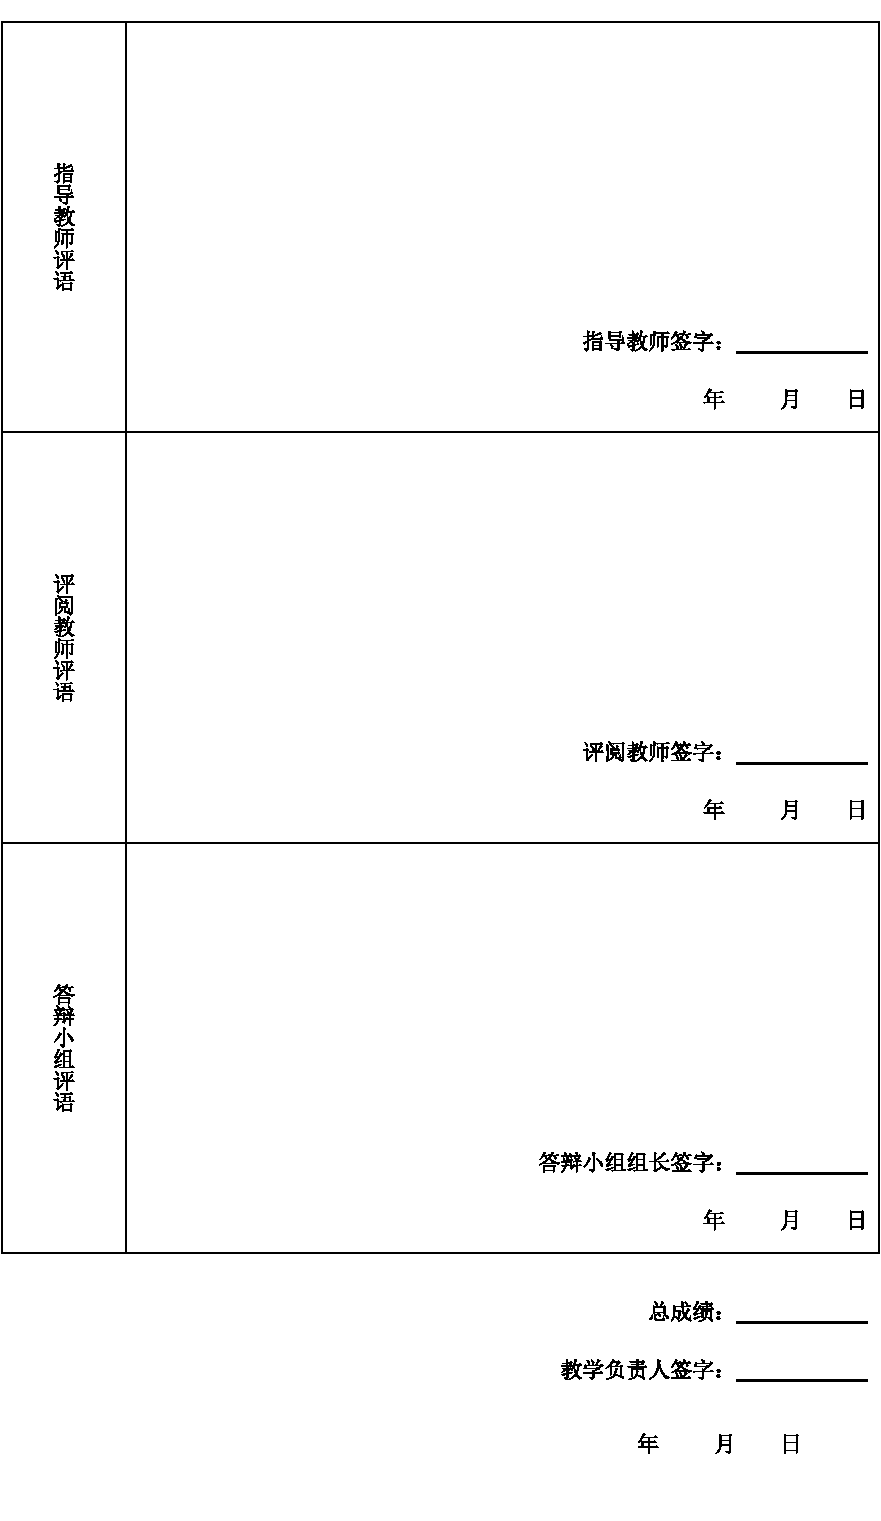
\includegraphics[width=0.95\linewidth]{record2-crop}
\end{figure*}

\end{document}
